%
% The first command in your LaTeX source must be the \documentclass command.
\documentclass[acmlarge,screen,dvipsnames]{acmart}
\usepackage[]{algorithm2e}
\usepackage{subcaption}

\usepackage[normalem]{ulem}  % for strike-through (\sout)
\input twmacros
%
% defining the \BibTeX command - from Oren Patashnik's original BibTeX documentation.
\def\BibTeX{{\rm B\kern-.05em{\sc i\kern-.025em b}\kern-.08emT\kern-.1667em\lower.7ex\hbox{E}\kern-.125emX}}
    
% Rights management information. 
% This information is sent to you when you complete the rights form.
% These commands have SAMPLE values in them; it is your responsibility as an author to replace
% the commands and values with those provided to you when you complete the rights form.
%
% These commands are for a PROCEEDINGS abstract or paper.
%\copyrightyear{2018}
%\acmYear{2018}
%\setcopyright{acmlicensed}
%\acmConference[Woodstock '18]{Woodstock '18: ACM Symposium on Neural Gaze Detection}{June 03--05, 2018}{Woodstock, NY}
%\acmBooktitle{Woodstock '18: ACM Symposium on Neural Gaze Detection, June 03--05, 2018, Woodstock, NY}
%\acmPrice{15.00}
%\acmDOI{10.1145/1122445.1122456}
%\acmISBN{978-1-4503-9999-9/18/06}

%
% These commands are for a JOURNAL article.
\setcopyright{acmcopyright}
\acmJournal{JOCCH}
\acmYear{2018}\acmVolume{37}\acmNumber{4}\acmArticle{111}\acmMonth{8}
\acmDOI{10.1145/1122445.1122456}

%
% Submission ID. 
% Use this when submitting an article to a sponsored event. You'll receive a unique submission ID from the organizers
% of the event, and this ID should be used as the parameter to this command.
%\acmSubmissionID{123-A56-BU3}

%
% The majority of ACM publications use numbered citations and references. If you are preparing content for an event
% sponsored by ACM SIGGRAPH, you must use the "author year" style of citations and references. Uncommenting
% the next command will enable that style.
%\citestyle{acmauthoryear}

%
% end of the preamble, start of the body of the document source.
\begin{document}

%
% The "title" command has an optional parameter, allowing the author to define a "short title" to be used in page headers.
\title[Digital workflow for creating 3D puzzles]%
      {\KR{let's change title to have a different name from the previous publication}Digital workflow for creating 3D puzzles to engage audiences in the interpretation of archaeological artefacts}
%
% The "author" command and its associated commands are used to define the authors and their affiliations.
% Of note is the shared affiliation of the first two authors, and the "authornote" and "authornotemark" commands
% used to denote shared contribution to the research.
\author{Karina Rodriguez Echavarria}
\email{K.Rodriguez@brighto.ac.uk}
\orcid{0000-0002-8679-1602}
\affiliation{%
  \institution{Centre for Secure, Intelligent and Usable Systems, University of Brighton}
  \city{Brighton}
  \country{United Kingdom}
}

\author{Myrsini Samaroudi}
\affiliation{%
  \institution{Centre for Secure, Intelligent and Usable Systems, University of Brighton}
  \city{Brighton}
  \country{United Kingdom}
  }

\author{Tim Weyrich}
\affiliation{%
  \institution{University College London}
  \city{London}
  \country{United Kingdom}
}


%
% By default, the full list of authors will be used in the page headers. Often, this list is too long, and will overlap
% other information printed in the page headers. This command allows the author to define a more concise list
% of authors' names for this purpose.
\renewcommand{\shortauthors}{K. Rodriguez, M. Samaroudi \& T. Weyrich}

%
% A "teaser" image appears between the author and affiliation information and the body 
% of the document, and typically spans the page. 
\begin{teaserfigure}
\centering
\subcaptionbox{3D scanned model of archaeological artefact\label{step1}}
 {\raisebox{0.3\height}{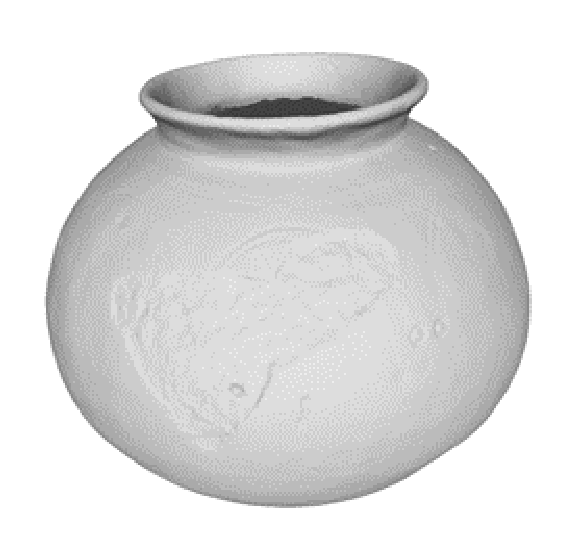
\includegraphics[width=.23\linewidth]{images/potscanned}}}
 \subcaptionbox{Generate puzzle pieces and core\label{step2}}
 {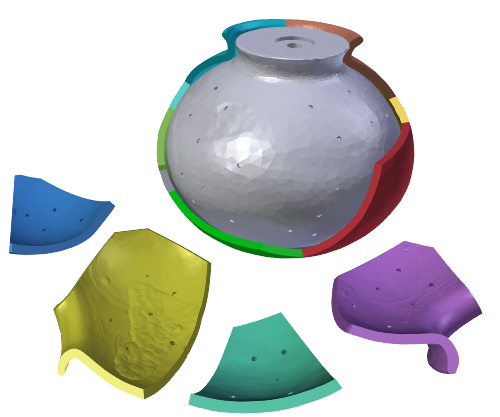
\includegraphics[width=.40\linewidth]{images/allpieces}}
 \subcaptionbox{Fabricated puzzle for museum exhibit\label{step3}}
  {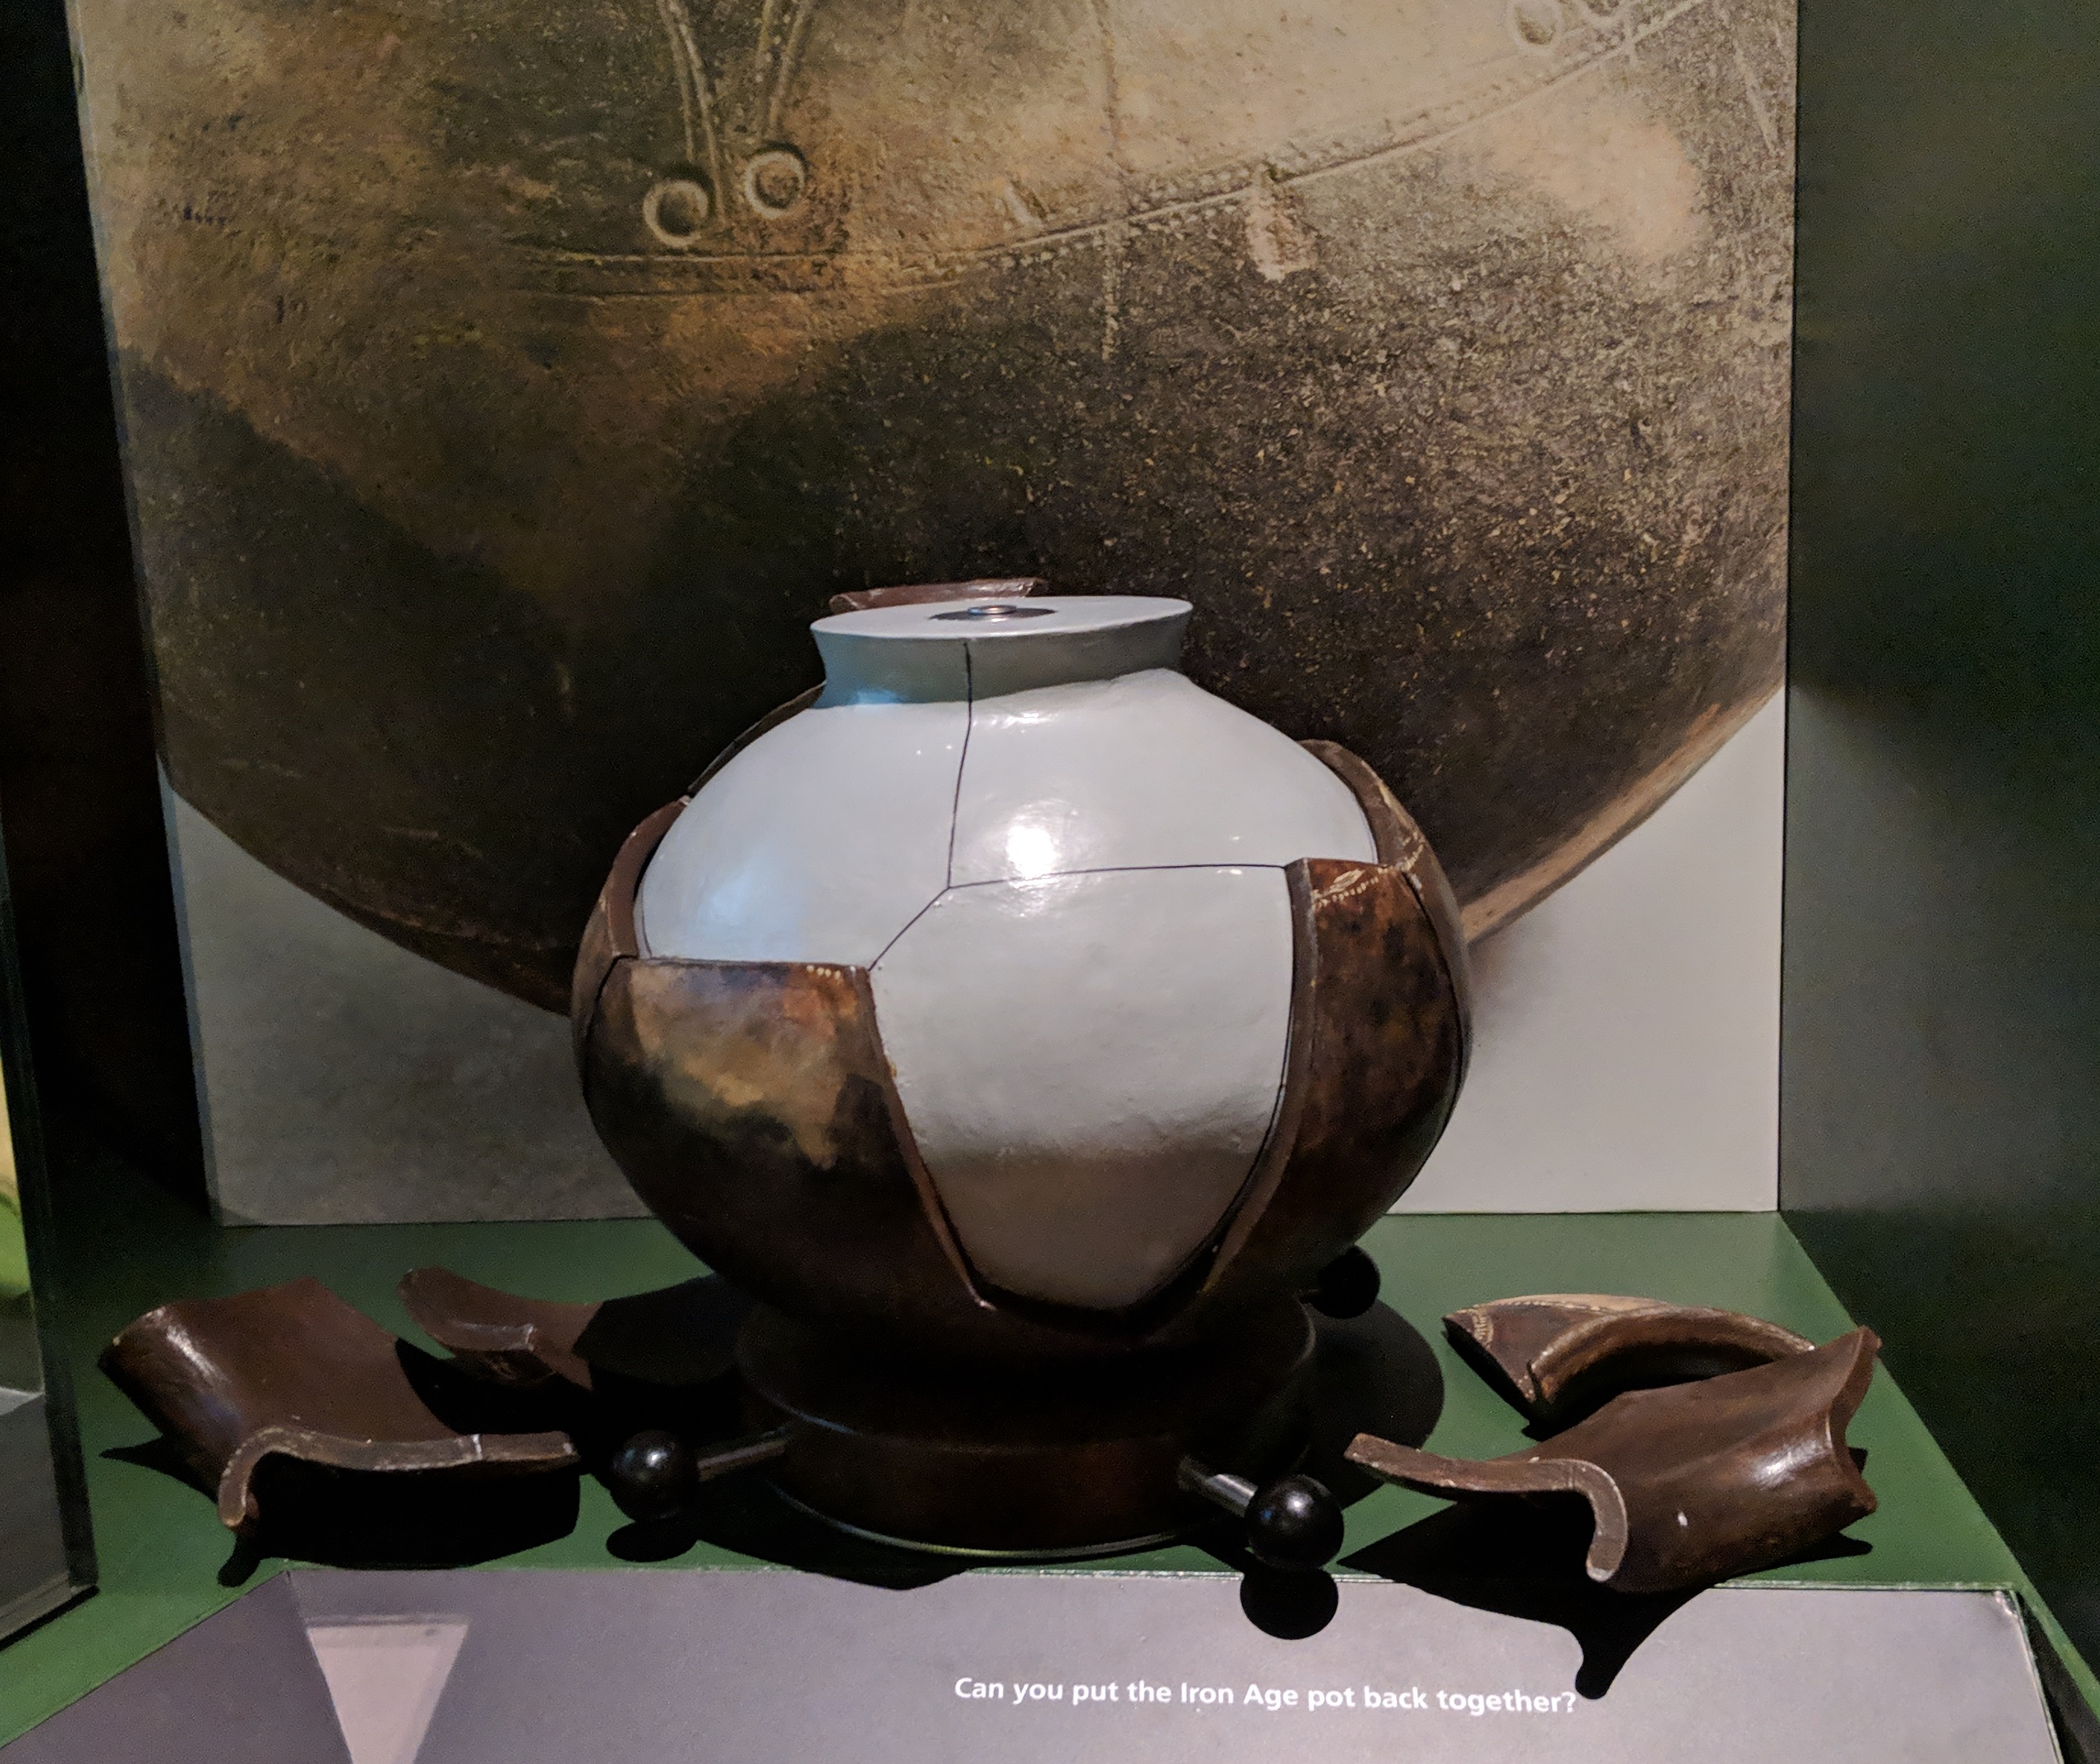
\includegraphics[width=.35\linewidth]{images/exhibitmuseum}}
  \caption{Workflow for the development of physical puzzle of pottery archaeological artefacts}
  \label{fig:teaser}
\end{teaserfigure}
%
% The abstract is a short summary of the work to be presented in the article.
\begin{abstract}
3D physical puzzles are typically used to engage audiences in the
interpretation of archaeological artefacts in a museum \KRedit[exhibition]{gallery}. The reason for this is that a puzzle can be seen as a game but also as a
complex activity that archaeologists undertake to re-assemble
fragments. The contribution of this paper is a novel \KRedit[digital]{} worfklow
for the design and fabrication of \KRedit[3D]{physical} heritage puzzles. The input to
the workflow is an authentic artefact from a heritage collection,
which is then digitised using technologies such as 3D scanning and 3D
modelling. Thereafter, a puzzle generator produces the \KRedit[3D]{} puzzle
pieces using a cell fracture algorithm and generates a set of puzzle
pieces (female) and a single core piece (male) for
fabrication. Finally, the pieces are fabricated using 3D printing
technology and post-processed to facilitate the puzzle assembly. \KR{The following is to specific and needs to be rephrased to be more generic while keeping the saltdean pot at the centre of the deployment of the full workflow} To
demonstrate the workflow, we deploy the proposed method to create a 3D
puzzle of an artefact, the Saltdean urn, for the Archaeological
Gallery of the Brighton Museum and Art Gallery. The significance of
this research is that it eases the task of creating puzzle-like
activities and maintaining them within a busy museum gallery.
\end{abstract}

%
% The code below is generated by the tool at http://dl.acm.org/ccs.cfm.
% Please copy and paste the code instead of the example below.
%
 \begin{CCSXML}
<ccs2012>
<concept>
<concept_id>10010147.10010371.10010396</concept_id>
<concept_desc>Computing methodologies~Shape modeling</concept_desc>
<concept_significance>500</concept_significance>
</concept>
<concept>
<concept_id>10010147.10010371.10010396.10010398</concept_id>
<concept_desc>Computing methodologies~Mesh geometry models</concept_desc>
<concept_significance>100</concept_significance>
</concept>
<concept>
<concept_id>10010405.10010432.10010439.10010440</concept_id>
<concept_desc>Applied computing~Computer-aided design</concept_desc>
<concept_significance>300</concept_significance>
</concept>
<concept>
<concept_id>10010405.10010469.10010470</concept_id>
<concept_desc>Applied computing~Fine arts</concept_desc>
<concept_significance>300</concept_significance>
</concept>
</ccs2012>
\end{CCSXML}


\ccsdesc[500]{Computing methodologies~Shape modeling}
\ccsdesc[100]{Computing methodologies~Mesh geometry models}
\ccsdesc[300]{Applied computing~Computer-aided design}
\ccsdesc[300]{Applied computing~Fine arts}


%
% Keywords. The author(s) should pick words that accurately describe the work being
% presented. Separate the keywords with commas.
\keywords{cultural heritage, 3D printing, galery design}


  %\caption{a) 3D scanned model of pottery urn artefact; b) 3D model of puzzle pieces of reconstructed urn; c) printed parts of the puzzle }



%
% This command processes the author and affiliation and title information and builds
% the first part of the formatted document.
\maketitle




%-------------------------------------------------------------------------
\section{Introduction}

The technological developments over the last years in 3D printing along with the
attention that its applications have attracted from various
communities, have resulted in making digital fabrication a popular
topic of research, practice and discussion. Even though there is still
a need to deal with several related obstacles, such as design
knowledge, cost and available materials, before the widespread
adoption of digital fabrication in people's everyday lives, the
Cultural Heritage (CH) domain has proved to be a valuable field to try
digital fabrication technologies. These technologies have already been
implemented in a variety of processes in the CH sector from
conservation and exhibition planning to packaging and creative or
educational activities
\cite{Neely2013,Scopigno2014,Neumuller2014,Scopigno2015}.

This paper is concerned with the development of an application of
digital fabrication which aims to contribute to the educational and
communicational aspect of the CH experience. In particular, it
examines how digital 3D models of artefacts can be re-purposed in
creative ways in order to expand the benefits of the digitisation
process. As such, the paper proposes the playful use of a 3D puzzle to
enable users to experience the physical pieces or shards of a pot in a
similar way that archaeologists do when uncovering and synthesizing an
artefact found at an excavation site. This requires digitally breaking
a 3D shape into pieces and physically fabricating them in such a way
that the puzzle can be easily re-assembled.

The technical contribution of this paper is a workflow for generating
and fabricating the physical puzzle when the given input is an
authentic museum artefact. The design of the 3D puzzle is driven by
the main requirement which is to be easily assembled by a young person
or child. The workflow is deployed with a late Iron Age burial urn
from the area of Sussex (UK) - a significant object from the Brighton
Museum and Art Gallery collection. The generated puzzle \KRedit[will be]{has been}
incorporated into the archaeology \KRedit[exhibition at the museum and is
targeted]{gallery in order} to enhance young audiences' visiting experience while
engaging them in an educational activity.

In addition\TW{describe that we explore different fracture patterns}

The paper is organised as follows. Section~\ref{related} discusses
relevant work in the field including 3D printing technologies to
communicate cultural heritage information and engage
audiences. Section~\ref{requirements} introduces the particular
artefact which drove the requirements for the development of the
puzzle generating workflow and the audience of the
application. Section~\ref{workflow} then presents the proposed
workflow for the design and fabrication of the puzzle, including the
3D scanning of the artefact, its reconstruction and an algorithm for
generating the puzzle. Section~\ref{eva} discusses the evaluation of
the application and the advantages of the adopted approach. Finally,
section~\ref{conclusions} presents discussions and conclusions.

%-------------------------------------------------------------------------
\section{Related work}
\label{related}

\subsection{Digital fabrication to communicate CH information}

Digital fabrication technologies comprise a combination of
programmable digital tools, processes, materials and equipment which
allow the creation of physical objects of complexities not achievable
by traditional manufacturing processes.

The interest from the CH community in these technologies is high as
they offer the ability to manipulate the digital representation of an
artefact in creative ways. In addition, these technologies enable a
high-level of customisation when producing physical objects in a
variety of resolutions, materials, colours and densities. Another
important advantage of digital fabrication includes the possibility
for multiple replication and/or production in a cost effective way,
while ``future-proofing'' the information related to the artefact
itself. Hence, these technologies are driving new trends for the
mass-customisation of CH objects and experiences.

The term ``smart'' replicas has also become popular over the recent
years. This refer to the possibility of combining the physical object
with further layers of interpretative multimedia information
\cite{Capurro2015,Marshall2016}.

Moreover, digital fabrication applications to support the
interpretation and communication of CH can be found in many heritage
organisations around the world. These examples include applications,
such as the full 3D print of the Sarcophagus of the Spouses from the
Villa Giulia Etruscan Museum, which can support visitors in having a
more holistic approach (by vision and touch) for the interpretation of
an artefact~\cite{Guidazzoli2014}.

Another example involves audiences in scanning objects and mixing 3D
models to produce hybrid artefacts by using digital fabrication. These
activities can be oriented to people with knowledge of 3D tools, such
as artists participating in 3D scanning and printing Hackathons
\cite{Mullaney2012,Neely2013}. However, some institutions
(e.g. British Museum and the Art Institute of Chicago) deploy 3D
printing in order to involve groups in workshops for non-experts. Such
groups include teachers, teenagers and families who engage with the
museums' collections through 3D technology
\cite{BritishMuseum2016,Neely2015,Miles2015}.

Other examples employ 3D printed artefacts in educational programmes
for children. The American Museum of Natural History asked students to
capture and replicate dinosaur fossils from the museum's paleontology
collections in order to synthesise a dinosaur and learn to think like
paleontologists~\cite{AMNH2013}. Another application is a megalithic
freestanding stone from Wales (UK) that was 3D printed in the form of
a vertical puzzle that could be assembled by children using a central
pillar~\cite{Miles2015}.

Visually impaired audiences as well as the elderly constitute groups
that can also benefit greatly from digital fabrication. Tooteko
facilitates the navigation on an architectural 3D printed facade,
allowing blind users to listen to audio descriptions
\cite{DAgnano2015}. 3D printed reliefs, with complementing interactive
applications, support visually impaired users to feel paintings and
natural history exhibits~\cite{Reichinger2016a,Samaroudi2017}.

At the same time, digitally fabricated artefacts can work as
engagement vehicles for elder audiences or trauma survivors while
experiencing the ``healing'' properties of object handling and
reminiscence~\cite{PleaseTouch2016}.

Alternative uses of replicas include the production of edible
artefacts, such as the ones created at the MediaLab of The
Metropolitan Museum of Art in New York, aiming to support the
understanding of artefacts by providing a multisensorial experience to
visitors~\cite{Tang2015}. More ``traditional'' examples can be found
in museums' shops, where replicas are sold as souvenirs or
decorative/collection objects~\cite{Young2017}.

Lastly, replicas have also served purposes related to the repatriation
of original artefacts. In these cases, replicas are kept in the
possession of the organisation while the original artefact returns to
its possessor (the opposite can happen as well)~\cite{Hollinger2013}.
 
The breadth and spread of applications demonstrates i) the wide
variety of experiential frameworks to provide people with the
opportunity to ``meet'' and ``feel'' culture in alternative ways, and
ii) the potential of digital fabrication technology to support the
interpretation of a CH object and engage audiences. The development of
digitally fabricated puzzles for audiences is a novel contribution to
the wider efforts in this area.
 
\subsection{Design challenges and relevant cases}
 
%This paper presents the design requirements and the workflow for the
%creation of a digitally fabricated puzzle pot.
%
The creation of a digitally fabricated puzzle can be achieved by
different methods and tools. An important overall requirement is the
generation of the puzzle pieces and the mechanism for their
assembly. The graphics' community has previously conducted relevant
research. For instance, the generation of interlocking parts from a 3D
model has been a popular topic over the last years, as it is not
currently possible to print a single object that is larger than the
working volume of a 3D printer. As such, various systems are proposed
which take as an input a 3D model and produce various smaller
interlocking pieces for 3D printing
\cite{Song:2015:POI:2797416.2797510,luo_chopper:_2012,klein_interlocking_2014,skouras_interactive_2015}. Moreover,
\cite{Xin:2011:MBP:2010324.1964992,Song:2012:RIP:2366145.2366147,sun_computational_2015}
present various algorithms for generating puzzles with interlocking
pieces, known as burr puzzles, from a 3D model.

\KRedit{Another relevant area of research is the simulation of fractures for 3D models. These fracturing effects are often used to display the breaking or destruction of objects or places in
computer games, virtual reality and the film industry. In this area, pre-defined fracture patterns are often computed, while more novel solutions focus on creating fast approximations which are computational efficienct and offer flexible control of fragment generation \cite{Schvartzman:2014:FAB:2556700.2556713,Hahn:2016:FAB:2897824.2925902,Zhu:2015:SRB:2809654.2766942,Muller:2013:RTD:2461912.2461934}. Of relevance to the heritage field is the geometric analysis of a datset of fracture patterns observed in wall paintings excavated at Akrotiri, Greece \cite{Shin:2012:ASF:2362402.2362404}. This analysis suggests pottery framents in a hierarchical fracture pattern where fragments break into two pieces recursively along cracks nearly orthogonal to previous ones.}


Most of the proposed solutions \KRedit{in the literature} aim to create puzzles consisting only
of the required individual pieces. However, in our case we aim to
create a permanent exhibit \KRedit[of a pottery vase]{} for a busy museum
gallery. \KRedit{As pottery is a common finding of archaeologist at an excavation site, we focus on this type of artefact, and the shape of its fragments when broken into shards or pieces. This type of artefact is also interesting as its reconstruction from
shards is a problem often faced by archaeologists.}. \KRedit[This means the puzzle should be easy to assemble by providing
a clue of the overall shape, and the concave nature of the shape means
that it can wrap around a static core element.]

\begin{figure}[H]
  \centering
  \subcaptionbox{Puzzle-pot from the Bristol Museum \& Art Gallery (UK), photo courtesy of Andrew Maxted}
  {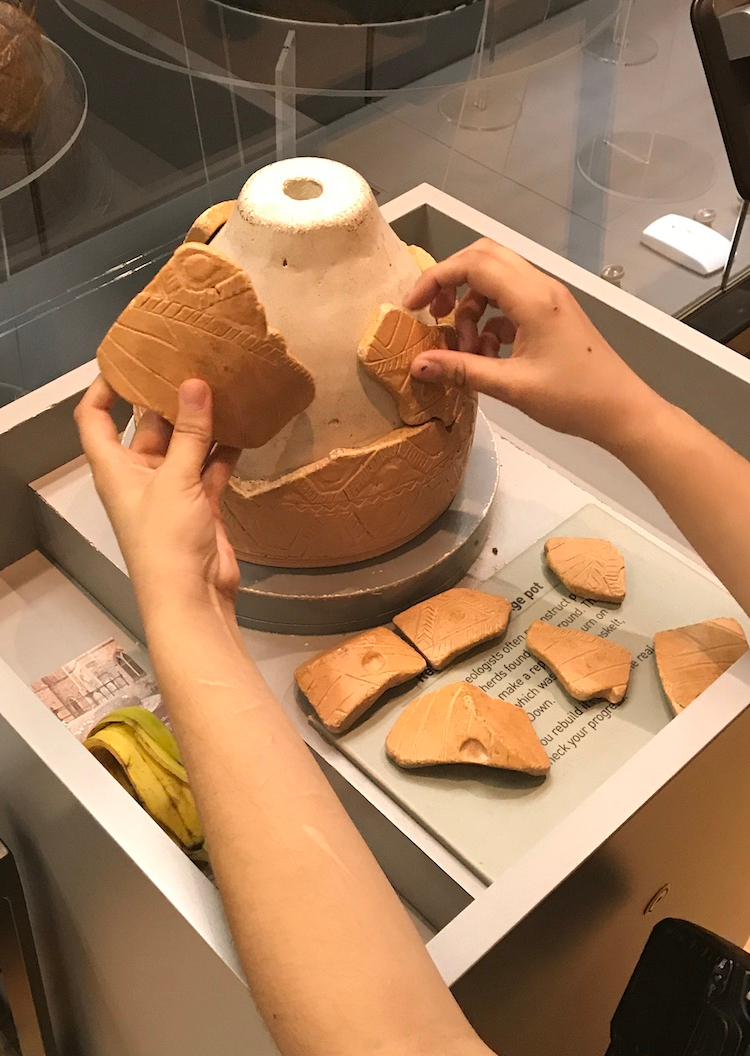
\includegraphics[width=0.35\linewidth]{images/uk}}
  \hspace{0.5in}
  \subcaptionbox{Puzzle-pot from Rez\'e Museum (France), photo courtesy of Theophane Nicola}
  {\includegraphics[width=0.35\linewidth]{images/france}}
  \caption{\label{fig:puz}Example of pottery puzzles in museums.}
\end{figure}

Similar examples of pottery puzzles in other museums (though without
deploying a fully digital workflow) are shown in
Figure~\ref{fig:puz}. As shown in the images, these puzzles require a
static element (the core) that provides a clue of the overall shape of
the pot. Moreover, the core helps \KRedit[the user to assemble the puzzle]{to secure the pieces in place} with
the use of magnets \KRedit{or other attachment mechanism which is placed both} on \KRedit[its]{the core's} surface and on each puzzle piece.

%Also, both the core and puzzle pieces are 3D printed making the exhibit and activity ``future-proof''. 


  

%Lastly, away from the puzzle context,~\cite{Barreau2014} propose a workflow to reconstruct a broken pot in order to display the existing shards for exhibition purposes.

\KRedit[The contribution of this paper is the proposed workflow to generate a
3D puzzle of a pot, which is a popular type of archaeological
artefact. This particular type of object is interesting as it is
widely found in all historic societies and its reconstruction from
shards is a problem often faced by archaeologists. The following
section will present more details on the particular object and the
design of the experience.]

%-------------------------------------------------------------------------
\section{The 3D puzzle experiential framework}
\label{requirements}
\KRedit[A funerary urn, shown in Figure~\ref{fig:pot}, from the collection of
the Brighton Museum and Art Gallery has been selected in order to
design an experience that will engage young audiences in assembling a
digitally fabricated 3D puzzle of the urn's replica.]{The motivation to develop the proposed workflow stemmed from the need to design an experience that will engage young audiences with the archaeological collection of the Brighton Museum and Art Gallery. Thus, the requirement was to design a 3D puzzle of a funerary urn, shown in Figure~\ref{fig:pot}.}
 The urn comes
from the cliff top at Saltdean, a coastal area near Brighton in
Sussex, UK. The pot has curvilinear designs which are usual in Sussex
in the two centuries BC, before the arrival of the Romans. The urn is
mostly brown and it seems that burnishing had been applied to its
surface to give it a ``leathery'' appearance. The Saltdean funerary
urn is a late Iron Age pot (probably 1st century BC) which was thrown
on a wheel~\cite{Toms1912}. It possibly reflects influences from
Belgian tribes and people from Brittany who had moved into the area
and introduced the use of the potter's wheel in south
Britain~\cite{Harding1974,Cunliffe1978,Adkins1982,Cunliffe1995}.
%
\begin{figure}[H]
  \centering
  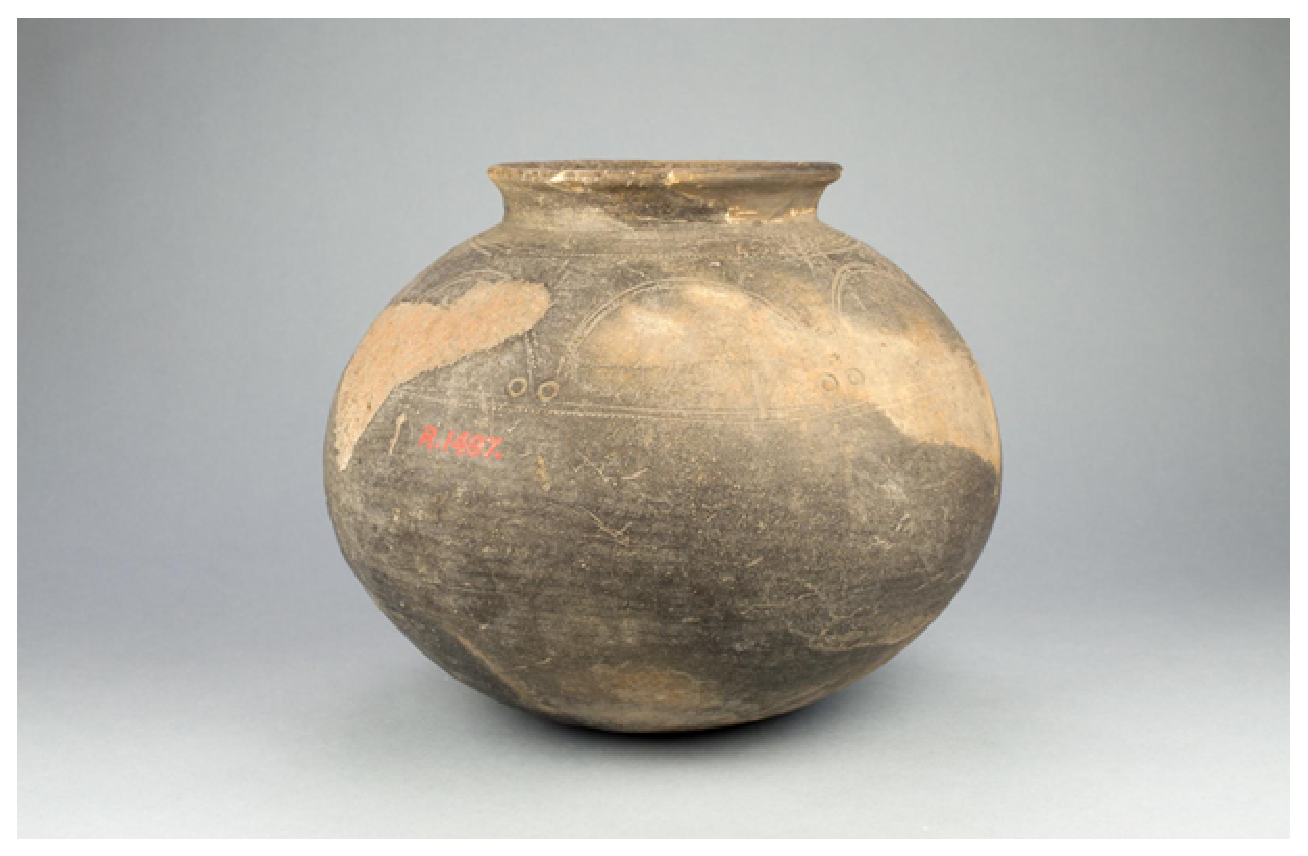
\includegraphics[width=0.6\linewidth]{images/pot}
  \caption{\label{fig:pot}
    Late Iron Age funerary urn from Saltdean, Sussex (UK)}
\end{figure}

\KRedit[The 3D puzzle will be a hands-on activity incorporated in the
Archaeological Gallery of the Brighton Museum and Art Gallery. The
puzzle will be placed along local findings of the Iron Age period and
will be close to the original artefact.]{ The
puzzle was designed to be placed as a hands-on activity along local findings of the Iron Age period and close to the original artefact in the new archaeology gallery.} The objective for the \KRedit[development of the puzzle]{hands-on activity} is to support young
audiences, and especially children, in having an interactive
experience with a heritage artefact in the form of an educational
activity or game. It \KRedit[will] also allows wider audiences to experience the
challenges linked to archaeological processes, such as reconstructing
a shape from a given group of shards or pieces. By assembling the
puzzle, audiences will engage with the exhibit, its physicality,
function and history, while acquiring new skills and gaining a better
understanding about the artefact itself.

\subsection{Requirements for the production of the digitally fabricated 3D puzzle}

The main design requirements with respect to the 3D puzzle were agreed
between the researchers and the exhibition designers taking into
account design guidelines about children's
puzzles~\cite{Smith2002}. These requirements included:
%
\begin{enumerate}
\item to have the urn height scaled-up to around 300 mm (the rest of
  the dimensions of the artefact were scaled-up proportionally);
\item to have a thickness of around 10 mm for each individual piece,
  as this was found suitable for easy handling by small hands;
\item to have approximately 10-12 pieces to assemble the puzzle. Thus,
  pieces should measure at least 50.8 mm across, as 6-8 year olds can
  handle pieces of this size;
\item to design a core piece which will be attached to a rotating
  wooden plate so that the user can easily spin the puzzle core to
  facilitate interaction (see Figure~\ref{fig:alexdesign});
\item to enable attachment of the individual puzzle pieces to the core
  via magnets. The magnets are inserted in blind holes in the puzzle
  pieces and in the solid core. The blind holes require to be in
  predetermined matching positions both in the pieces and core;
\item to cover each individual piece in a plaster-like finish and
  paint it to disguise the magnets, provide better texture feeling and
  a more realistic appearance.
\end{enumerate} 

\begin{figure}[H]
  \centering
  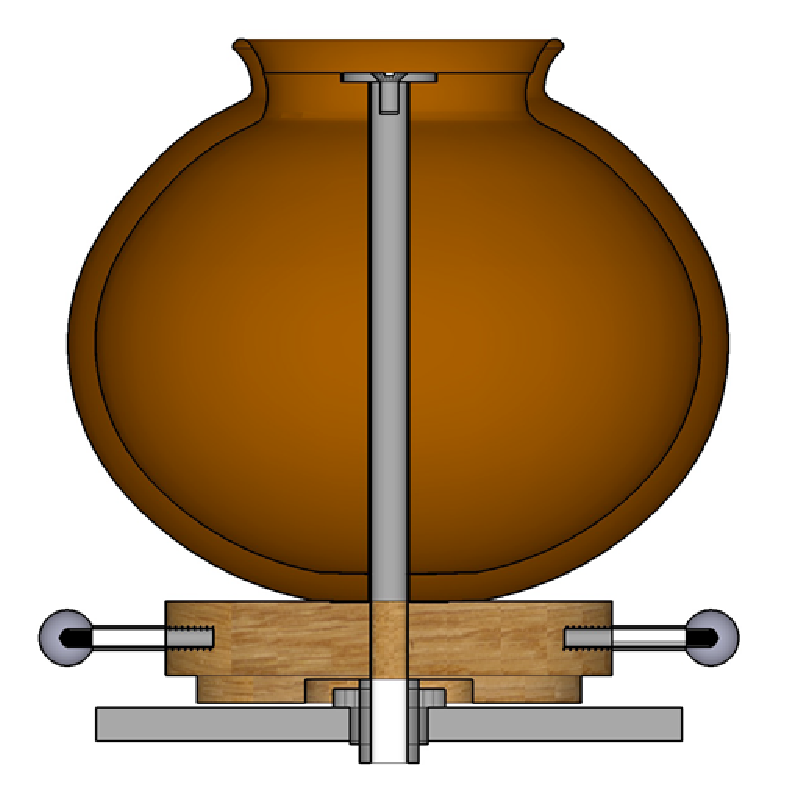
\includegraphics[width=0.5\linewidth]{images/alexdesign}
  \caption{\label{fig:alexdesign}%
    Design of puzzle core piece on its rotating base, design courtesy of Alex Hawkey}
\end{figure}

When discussing with the designer of the museum, it was acknowledged
that such requirements could be addressed by using alternative
mechanisms to digital fabrication technologies providing similar
durability and quality. However, it was deemed that the digital
workflow will enable to future-proof such exhibit for replacing parts
in a cost-effective manner.

\subsection{Audience}

The target group for this puzzle activity are young people, in
particular children between the age of 6 and 12 years old. This age
frame is considered as appropriate in terms of integrating a specific
type of interpretation as interpretative means can be different for
younger or older children~\cite{Tilden1977}.

The selection of this particular group, whether it is families or
school children visiting the museum, has been recognised as an
important part of most CH organisations' audiences. Children appear to
be amongst the people who can benefit the most from CH experiences
with the deployment of replicas~\cite{Cabral2013,Neely2015,Miles2015}.

Furthermore, official numbers (in the ``Overview of data in the
Museums, Libraries and Archives Sector''~\cite{Matty2004}) confirm
that most people who visit a museum/CH institution in the UK belong to
a family group or a school group. Hence, the Brighton Museum and Art
Gallery has a high numbers of families and school children visiting
its premises. Moreover a survey, realised in summer 2015 to record
visitors' opinions on the potential to exhibit the archaeological
collections of the museum, revealed that people would be interested in
hands-on children's activities~\cite{RoyalPavilionandMuseums2015}.

The following section will describe a digital fabrication workflow to
produce the 3D puzzle according to the specified requirements, along
with a proposed algorithm to semi-automate the design of such 3D
puzzles.

\section{Workflow for generating and fabricating a
  3D~puzzle of an archaeological pottery artefact}
\label{workflow}

The proposed workflow involves the following steps:
%
\begin{enumerate}
\item \KRedit[Acquiring]{Digtisation} and reconstructing the digital 3D model of the artefact and central core piece.
\KRedit{\item Generation of fracture pattern.}
\item Generation of the individual puzzle pieces.
\item Generation of \KRedit[matching blind-holes]{attachment mechanisms, such as matching blind holes,} both in the core and puzzle pieces.
\item 3D printing all puzzle pieces and core.
\item Post-processing of all puzzle pieces and core\KRedit[, which includes
  inserting the magnets]{, including adding attachments and painting.}
\item Assembling the puzzle into the final exhibit.
\end{enumerate}
%

\KRedit{The approach for generating solid surfaces for fabrication which underlies the proposed workshop combines algorithms for generating fracture patterns with constructive solid geometry (CSG) operations. CSG is a technique commonly used in solid modeling CAD systems. It allows to create a complex surface by using Boolean operators to combine simpler objects. 

The implementation of the workflow uses a mixture of tools and systems including modelling tools, C++ and OpenSCAD. OpenSCAD is a 
CSG engine based on the Computational Geometry Algorithms Library.  OpenSCAD is a free Computer Aided
Design (CAD) software which uses the Computational Geometry Algorithms
Library (CGAL) as its constructive solid geometry (CSG) engine. Its
script syntax is based upon functional programming philosophy which
allows to generate geometry using a functional approach.

The following subs-sections will describe each of the workflow stages in detail using the Saltdean pot as an example artefact.}


\KRedit[The following subs-sections will describe each of these stages in detail.]{}

\subsection{\KRedit[Acquiring the digital 3D model]{Digitisation and reconstruction of the heritage} artefact}

The acquisition of an artefact can be achieved through different
means, including 3D scanning and photogrammetry techniques. In this
case, the urn was scanned using the AICON Breuckmann 3D SmartScan
scanner. Given the shape of the urn with the narrowed neck above its
rounded body, the 3D scanning process captured the external surface of
the pot, but it was not possible to acquire the internal surface. The
resulting 3D model is shown in Figure~\ref{fig:teaser}-a after some
small holes were filled in.

In order to reconstruct the internal part of the urn which was not
acquired by the scanner, it was considered that the best approach was
to solidify the external wall \KRedit[at a suitable]{with a 10 mm} thickness using the 3D 
modelling tool Blender. Before doing this, the 3D model was scaled-up
to have a 300 mm height according to the design requirements. \KRedit[Then,
using the physics capabilities of Blender to simulate real-world
phenomena, the 3D model of the urn (whose base is not completely
straight) was placed on a plane in order to acquire a standing
position (see Figure~\ref{fig:blender}). Then, the top of the urns rim was removed in order to isolate the external shell of the urn.]{The resulting  3D model which will be used as input for the puzzle is shown in
  Figure~\ref{fig:reconstruction}-a.}
%
% \begin{figure}[h]
%   \centering
% % 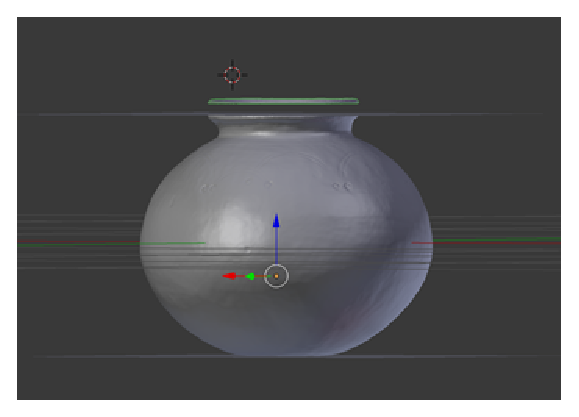
\includegraphics[width=0.45\linewidth]{images/blender1}
%   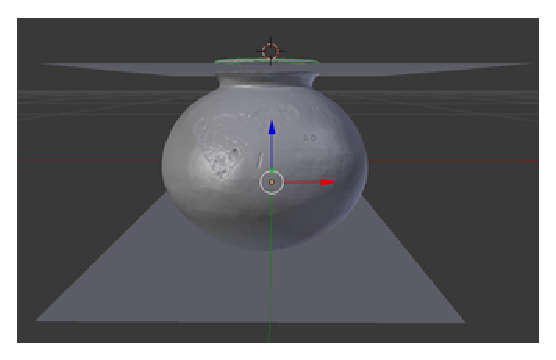
\includegraphics[width=0.6\linewidth]{images/blender2}
%   \caption{\label{fig:blender}
%     Perspective view of the urn with separated rim in Blender}
% \end{figure}

\KRedit[Subsequently, the external shell was solidified with a 10 mm thickness in Blender. This thickness is proportionally close to the scaled-up measurements of the artefact. Afterwards, two 3D models were produced:]{}

\KRedit[The urn without rim. The rim was later joined again with the urn and modeled to have a smooth feeling in order to produce the reconstructed 3D model of the pot (see  Figure~\ref{fig:reconstructiona}).]{}

\KRedit[The internal shell of the pot which constitutes the core of the puzzle. Thus, the faces of the internal shell were inverted it Meshlab and a plane was added to the top of the shape to create a watertight core (see Figure~\ref{fig:reconstructionb}).]{Afterwards, the central core piece is produced. This can be generated for any type of pottery puzzle by using a boolean operation. The resulting watertight is shown in Figure~\ref{fig:reconstructionb}. The core requires also of a through-hole along its height in order to fit it to the revolving base, as shown in the design in figure~\ref{fig:alexdesign}.}

\begin{figure}[h]
  \centering
  \subcaptionbox{3D model of the reconstructed urn\label{fig:reconstructiona}}
  {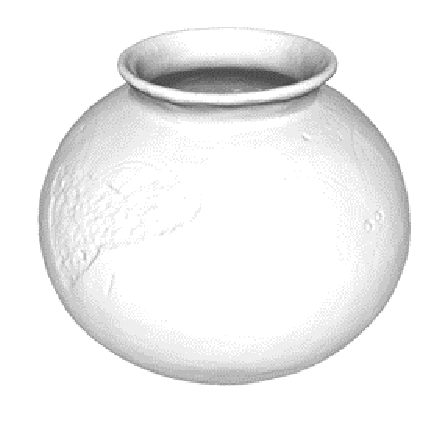
\includegraphics[width=0.45\linewidth]{images/3Dreconstruction}}
  \subcaptionbox{3D model of internal core of the puzzle\label{fig:reconstructionb}}
  {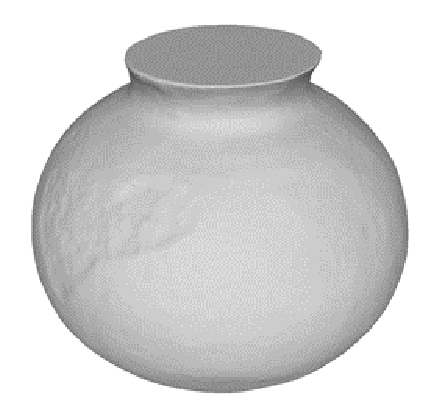
\includegraphics[width=0.45\linewidth]{images/core}}
  \caption{3D models used for puzzle generation}
\end{figure}

\greenBegin

\subsection{Generation of fracture patterns}
\TWboxed{say:
  \begin{itemize}
    \item we model fracture lines by projecting the pot's geometry onto
      a sphere; while this restricts us to mostly-spherical objects, it
      appears a reasonable approximation in our context.
    \item then describe different ways to create fractures
    \item visualise them by fracturing a perfect sphere, so we can
      show Blender fractures in the same way as our own:
      \begin{itemize}
      \item Figure 1: Blender, vs. hierarchical, but show the latter with
        straight lines (almost(?) zero amplitude)
      \item Figure 2: compare different fractal parameters
      \end{itemize}
      leave comparison of differently fractured models for the results
      section.
  \end{itemize}}


\begin{figure}[h]
  \centering
  \subcaptionbox{Voronoi fracture pattern}
  {\includegraphics[width=0.30\linewidth]{images/fractureblender}}
  \hspace{0.2in}
  \subcaptionbox{Hierarchical fracture pattern, m: 6, nitter: 6, jitter: 0.3, amplitude: 0.01, decay: 0.5, smoothing: 0.0}
  {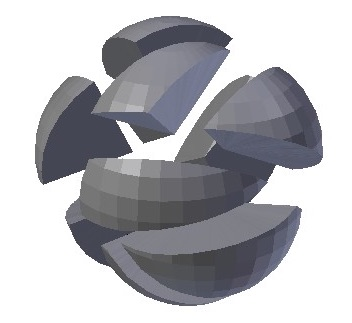
\includegraphics[width=0.30\linewidth]{images/fracturelowamplitude}}
  \hspace{0.2in}
  \subcaptionbox{Hierarchical fracture pattern, m: 6, nitter: 6, jitter: 0.3, amplitude: 0.1, decay: 0.5, smoothing: 1.0}
  {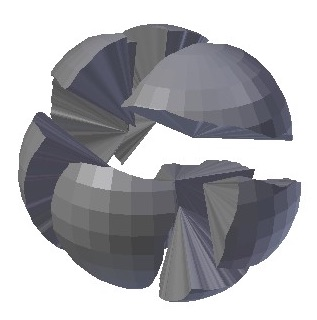
\includegraphics[width=0.30\linewidth]{images/fracturestandardsmooth}}
  \hspace{0.2in}\\
 \subcaptionbox{Hierarchical fracture pattern, m: 6, nitter: 6, jitter: 0.3, amplitude: 0.2, decay: 0.2, smoothing: 1.0}
  {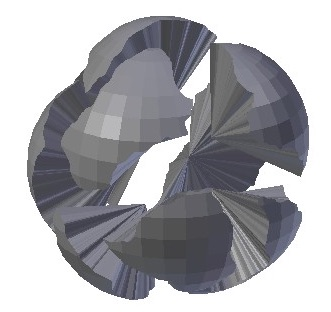
\includegraphics[width=0.30\linewidth]{images/fracturehighamplitude}}
  \hspace{0.2in}    
  \subcaptionbox{Hierarchical fracture pattern, m: 6, nitter: 6, jitter: 0.1, amplitude: 0.3, decay: 0.5, smoothing: 0.3}
  {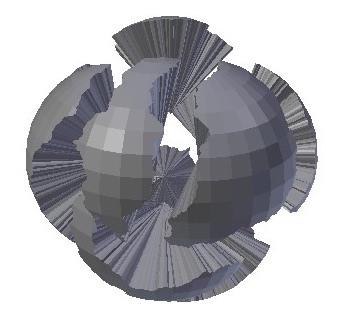
\includegraphics[width=0.30\linewidth]{images/fracturehighestamplitude}}    
  \caption{Fracture patterns}
\end{figure}



\KR{we can delete the following once the new section is in place.}To generate a puzzle pieces, firstly it is required to input a
randomly fractured geometry of a spherical polyhedron. To achieve
this, it is possible to use a cell fracture algorithm of a modeling
tool (e.g. Blender). The sphere is fractured into 14 pieces in this
case. However, it is possible to generate more or less pieces, if
smaller or larger puzzle pieces are desired.
%


\greenEnd

\subsection{Generating the individual puzzle pieces}

\KRedit[In order to generate the puzzle pieces, a semi-automated approach was
deployed using OpenSCAD software. OpenSCAD is a free Computer Aided
Design (CAD) software which uses the Computational Geometry Algorithms
Library (CGAL) as its constructive solid geometry (CSG) engine. Its
script syntax is based upon functional programming philosophy which
allows to generate geometry using a functional approach.]{}

\KRedit[The proposed approach takes as input the watertight 3D models of the
reconstructed urn (Figure~\ref{fig:reconstruction}-a) and core
(Figure~\ref{fig:reconstruction}-b), both generated in the previous
steps. The generator then produces:]{Once the fracture pattern has been generated, this is used to generate the puzzle pieces.}

\begin{figure}[h]
  \centering
  \subcaptionbox{3D model contained within all fragments of sphere\label{fig:spherea}}
  {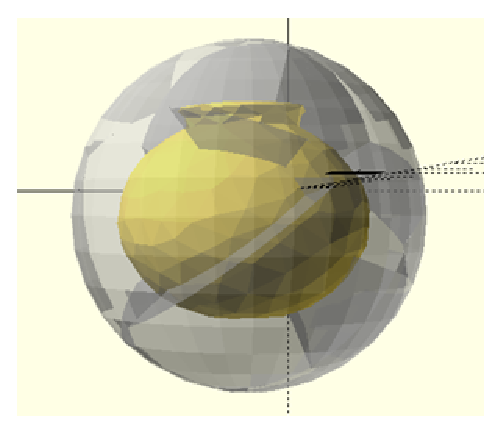
\includegraphics[width=0.30\linewidth]{images/sphere}}
  \hspace{0.2in}
   \subcaptionbox{3D model of reconstructed urn with fragment of the fractured sphere\label{fig:sphereb}}
   {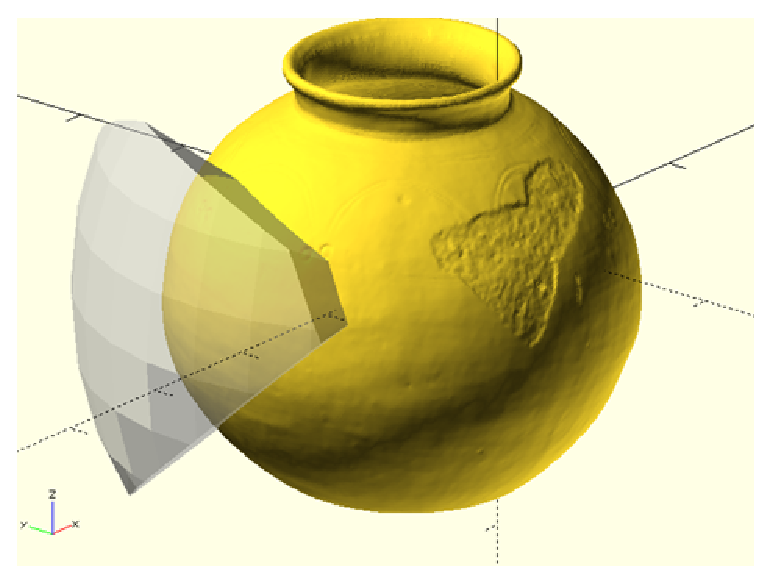
\includegraphics[width=0.30\linewidth]{images/intersection}}
   \hspace{0.2in}
  \subcaptionbox{Resulting 3D model of puzzle piece\label{fig:spherec}}
  {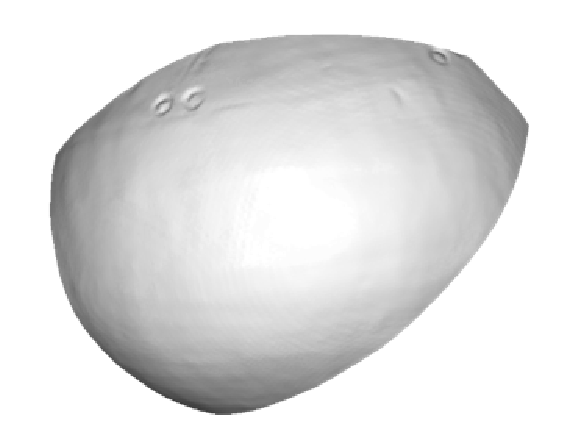
\includegraphics[width=0.30\linewidth]{images/puzzlepiece}}
    
    
    \caption{\KR{Need a better caption}Process of generating each puzzle piece using fracture pattern.}
\end{figure}

%


\KRedit[Boolean operations are used for generating the puzzle pieces and the
internal core with matching blind holes. These sets of operations,
including union, intersection and difference, are the basis of how
geometries are constructed in CAD systems.]{}

To generate each puzzle piece, the intersection operation is used. For
this, the 3D model is firstly translated to the centre of the fractured
sphere (see Figure~\ref{fig:spherea}). Thereafter, as shown in
Figure~\ref{fig:sphereb}, each \KR{do I use the word "section" before, not sure this is correct}section of the fractured sphere
is intersected with the 3D model of the reconstructed urn. The
intersection region of these two objects is defined as the set of all
points that are part of both objects. As a result, a puzzle piece is
produced as shown in Figure~\ref{fig:spherec}.
%

%

The algorithm iterates over all sections of the fractured sphere to
automatically produce all puzzle pieces. This process is repeated to
generate puzzle pieces at two different levels of detail so that they
can be used in subsequent operations.

\KRedit{For the Saltdean urn, we generated} 14 individual puzzle pieces. Six of these pieces are retained
  to be used for the base of the puzzle. The user will use this base
  as a reference when assembling the rest of the puzzle pieces. \KRedit[The
  remaining 8 pieces are generated with up to 6 holes each for
  fitting the magnets. and up to 60
  matching blind-holes distributed across the surface to fit the
  magnets.]


\subsection{Generating \KRedit[matching blind-holes]{attachments} both in the core and puzzle pieces}

Once all puzzle pieces have been produced, \KRedit[matching blind-holes]{it is necessary to generate attachments which will secure the puzzle pices to the core. Magnets are suitable attachments as they can be buried within the puzzle piece and core. However, other female/male attachments are possible as well. In this step, the attachments for the Saltdean urn} are
generated both for the individual puzzle pieces and the central core
to fit the magnets in. The blind-holes have consistent width and depth
which should be enough to hide the magnets in.

To generate the blind-holes across the surface, a set of points in 3D
space is given as an input. This set of points should offer full
coverage across the surface. The set can be randomly generated as
random points on a sphere. However, given the requirement to have a
specific number of holes for each piece, the positions were manually
determined to ensure an even distribution. Each point is then used to
generate a cylinder whose origin is the centre of the 3D model, as
illustrated in Figure~\ref{fig:cylinders}.
%
\begin{figure}[H]
  \centering
  \subcaptionbox{Cylinders generated using as input a set of points in 3D space\label{fig:cylinders}}
  {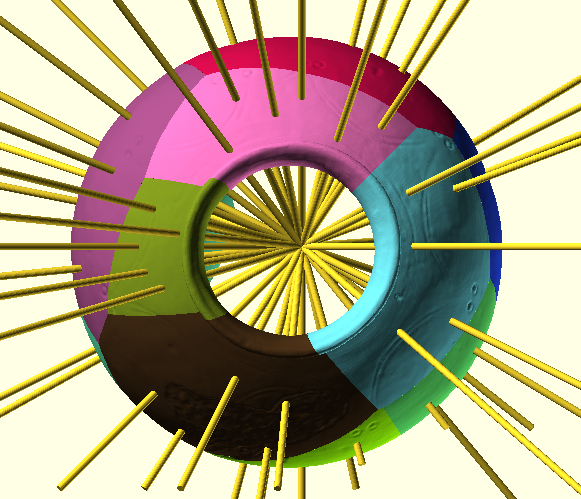
\includegraphics[width=0.45\linewidth]{images/allcylinders.jpg}}
  \subcaptionbox{Core with blind-holes across the surface\label{fig:coreholes}}
  {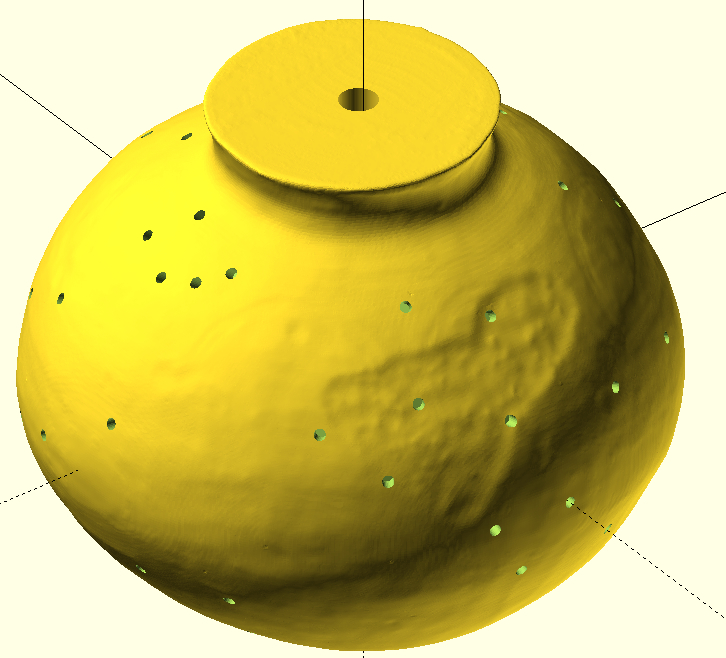
\includegraphics[width=0.45\linewidth]{images/coreholes.jpg}}
 \caption{Generating of matching holes for fitting magnets which will be the attachment mechanism for the Saltdean urn}
\end{figure}

The algorithm to create the blind-holes is based on the intersection
and difference operations. Hence, the algorithm can be described in
Algorithm~\ref{code}. This produces an intersection between the cylinder and \KRedit[a
simplified version of]{} the puzzle piece \KRedit[for speed purposes]{as shown in figure~\ref{fig:holesa}}. It then
translates the resulting geometry of the interaction towards the
origin by taking into account a thickness value. This code generates a
geometry, which will later become the hole, for each cylinder as shown
in Figure~\ref{fig:holesb}.
%
\begin{algorithm}
 \KwData{3D model of puzzle piece and set of 3D points}
 \SetKw{KwBy}{by}
 \KwResult{3D model of puzzle piece with blind holes}
   $points$: set of 3D points\;
   $3dmodel$: 3D model of puzzle piece simplified\;
   $thickness$: thickness of the blind hole\;
  \For{$i\gets0$ \KwTo length(points)}{ 
  $point$ = points[$i$]\;
  $unitvector$ = point/norm(point)\;
  translate($-unitvector$*$thickness$)
  intersection(3dmodel,cylinder($point.x$,$point.y$,$point.z$))\; 
  }
  \caption{\label{code}%
    Algorithm pseudo-code to generate geometries for blind-holes in puzzle pieces}
\end{algorithm}


The generated geometries are then used to produce the
blind-holes. This is achieved by using the difference operation
between the 3D puzzle piece and the generated geometry (see
Figure~\ref{fig:holesc}). The same process is repeated for all
the puzzle pieces \KRedit[. This step produces all puzzle pieces with]{to produce} the
required blind holes (see Figure~\ref{fig:teaser}-c).
%
\begin{figure}[h]
  \centering
    \subcaptionbox{Puzzle piece with cylinder for blind-holes\label{fig:holesa}}
     {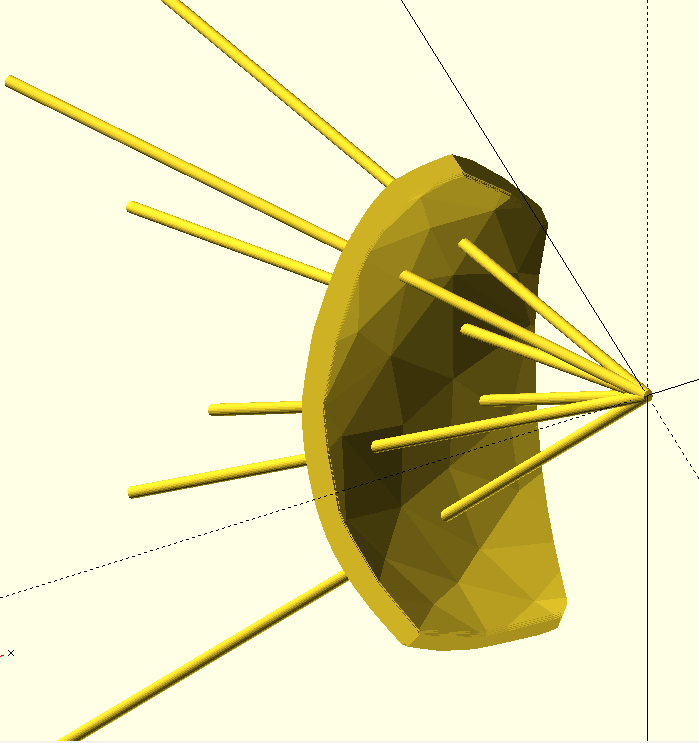
\includegraphics[width=0.33\linewidth]{images/holes1.jpg}}
  \hspace{0.3in}
    \subcaptionbox{Puzzle piece with geometry generated for the creation of each blind-hole\label{fig:holesb}}
    {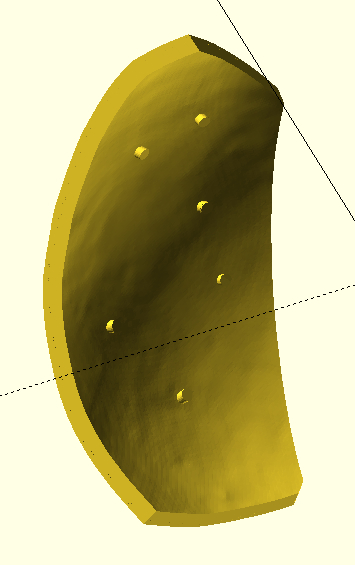
\includegraphics[width=0.22\linewidth]{images/holes2.jpg}}
  \hspace{0.3in}
    \subcaptionbox{Puzzle piece with blind-holes\label{fig:holesc}}
    {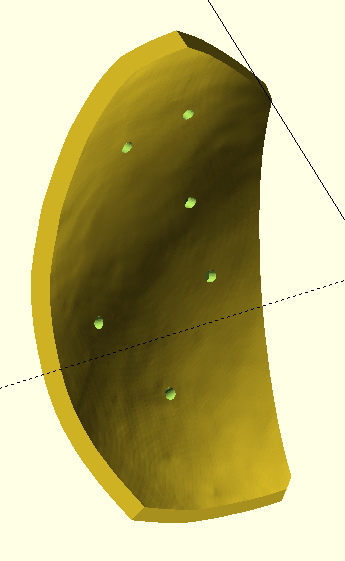
\includegraphics[width=0.22\linewidth]{images/holes3.jpg}}
      
  \caption{Generating blind holes for each puzzle piece}
\end{figure}

Furthermore, a similar process is repeated for generating the
blind-holes in the \KRedit{central} core piece using the same 3D points. However, this
time the direction in which the intersected geometry is translated is
reversed. The resulting geometry is shown in
Figure~\ref{fig:coreholes}. \KRedit[The core also requires a through central
hole for fixing it to the rotating base.]
%

\begin{figure}[H]
  \centering
  \subcaptionbox{3D printed prototypes for validation\label{fig:test}}
  {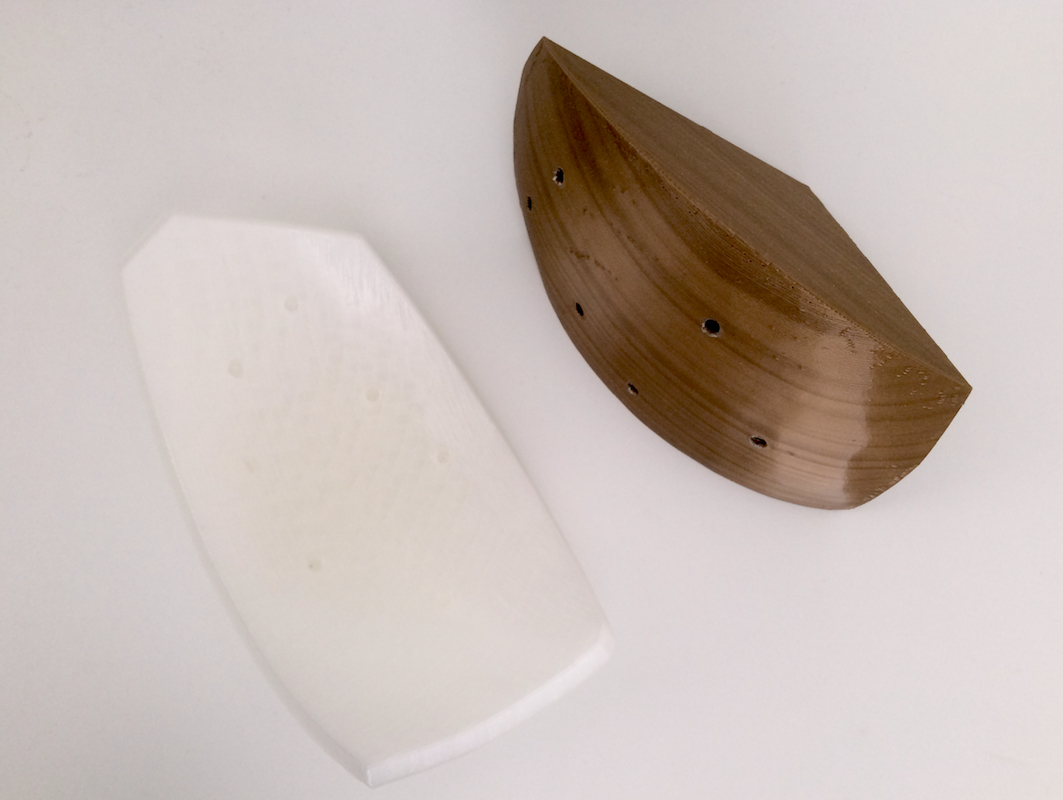
\includegraphics[width=0.45\linewidth]{images/coreANDpiece}}
  \subcaptionbox{Colour and texture for the puzzle pieces\label{fig:col}}
  {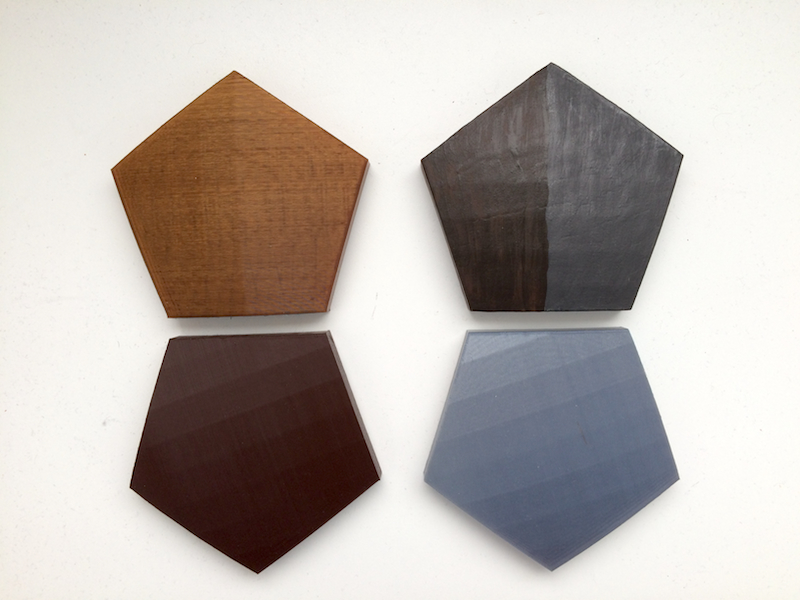
\includegraphics[width=0.45\linewidth]{images/colours}}

  \caption{
    Prototyping was performed before full fabrication of puzzle}
\end{figure}


\subsection{3D printing puzzle pieces and core}
\KRedit[Before printing all puzzle pieces,]{Before proceeding to fabricate the whole 3D puzzle, we underook a prototyping phase. In this,} a sample set of pieces were 3D
printed to validate the dimensions of the \KRedit[holes]{design} as well as to check
whether the overall dimensions and weight were suitable for the
purposes of the activity (see Figure~\ref{fig:test}). \KRedit[Some minor]{Various}
adjustments were made to the dimensions of the \KRedit[holes]{design} to take into
account \KRedit{tolerances caused by other parts and} the thickness of the printed layers for the print. This
thickness usually depends on the nozzle size and the machine and will
vary for different printing technologies.
%


Finally, all the puzzle pieces were 3D printed, as shown in
Figure~\ref{fig:allprinted}. Although the core could be printed all at
once, it was split into \KRedit{eight}[four] sections to achieve better printing
quality (and less supporting material) by allowing each section to be
positioned flat on the printer's bed).

\begin{figure}[h]
  \centering

  \centering
  \subcaptionbox{Printed puzzle pieces and central core.\label{fig:allprinted}}
  {\includegraphics[width=0.48\linewidth]{images/allprintedpieces}}
  \subcaptionbox{Post-processed puzzle pieces and central core.\label{fig:assembled}}
  {\includegraphics[width=0.41\linewidth]{images/allprintedpiecesassembled}}\\
   \subcaptionbox{Painted and assembled puzzle at the museum gallery.\label{fig:allprintedassembled}}
  {\includegraphics[width=0.48\linewidth]{images/exhibitmuseumassembled}}
    \caption{Fabricated puzzle pieces and central core generated by proposed workflow.}
\end{figure}

All pieces were printed in PLA (Polylactic Acid) filament on a FDM
(Fused Deposition Modeling) 3D printer at a 0.2mm layer thickness with
an infill value of 12\%. The core piece was printed at a 0.4 mm layer
thickness.


\subsection{Post-processing all puzzle pieces and core}

Post-processing of the puzzle pieces and the core includes removing
the supporting material around the pieces and sanding any rough
surfaces. Then, the magnets are inserted in holes at the back of each
puzzle piece and on the core. The holes are covered afterwards with
plaster and sanded accordingly.

When the plaster has dried, a coating using a mixture of PVA
(Polyvinyl acetate) glue, marble powder and water is applied on the
puzzle pieces and core in order to provide a ceramic-like
texture. Figure~\ref{fig:assembled} \KRedit[demonstrates the samples that were 3D printed using PLA filaments in different colours. The sample on the top right of the image has been chosen for the puzzle pot. The sample has been coated with the described mixture and painted using acrylic colours. The pieces are currently being post-processed to achieve the same visual quality as the samples.]{demonstrates the 3D puzzle assembled once all the pieces and the core have been post-processed. Afterwards, an artist painted the pieces using the colours tested and the final interactive exhibit is then placed at the musuem gallery (see Figure~\ref{fig:allprintedassembled} ).}


\section{Results}
\KR{need to add something here about the generalisation of the results. Tim can you advice?}
\begin{figure}[h]
  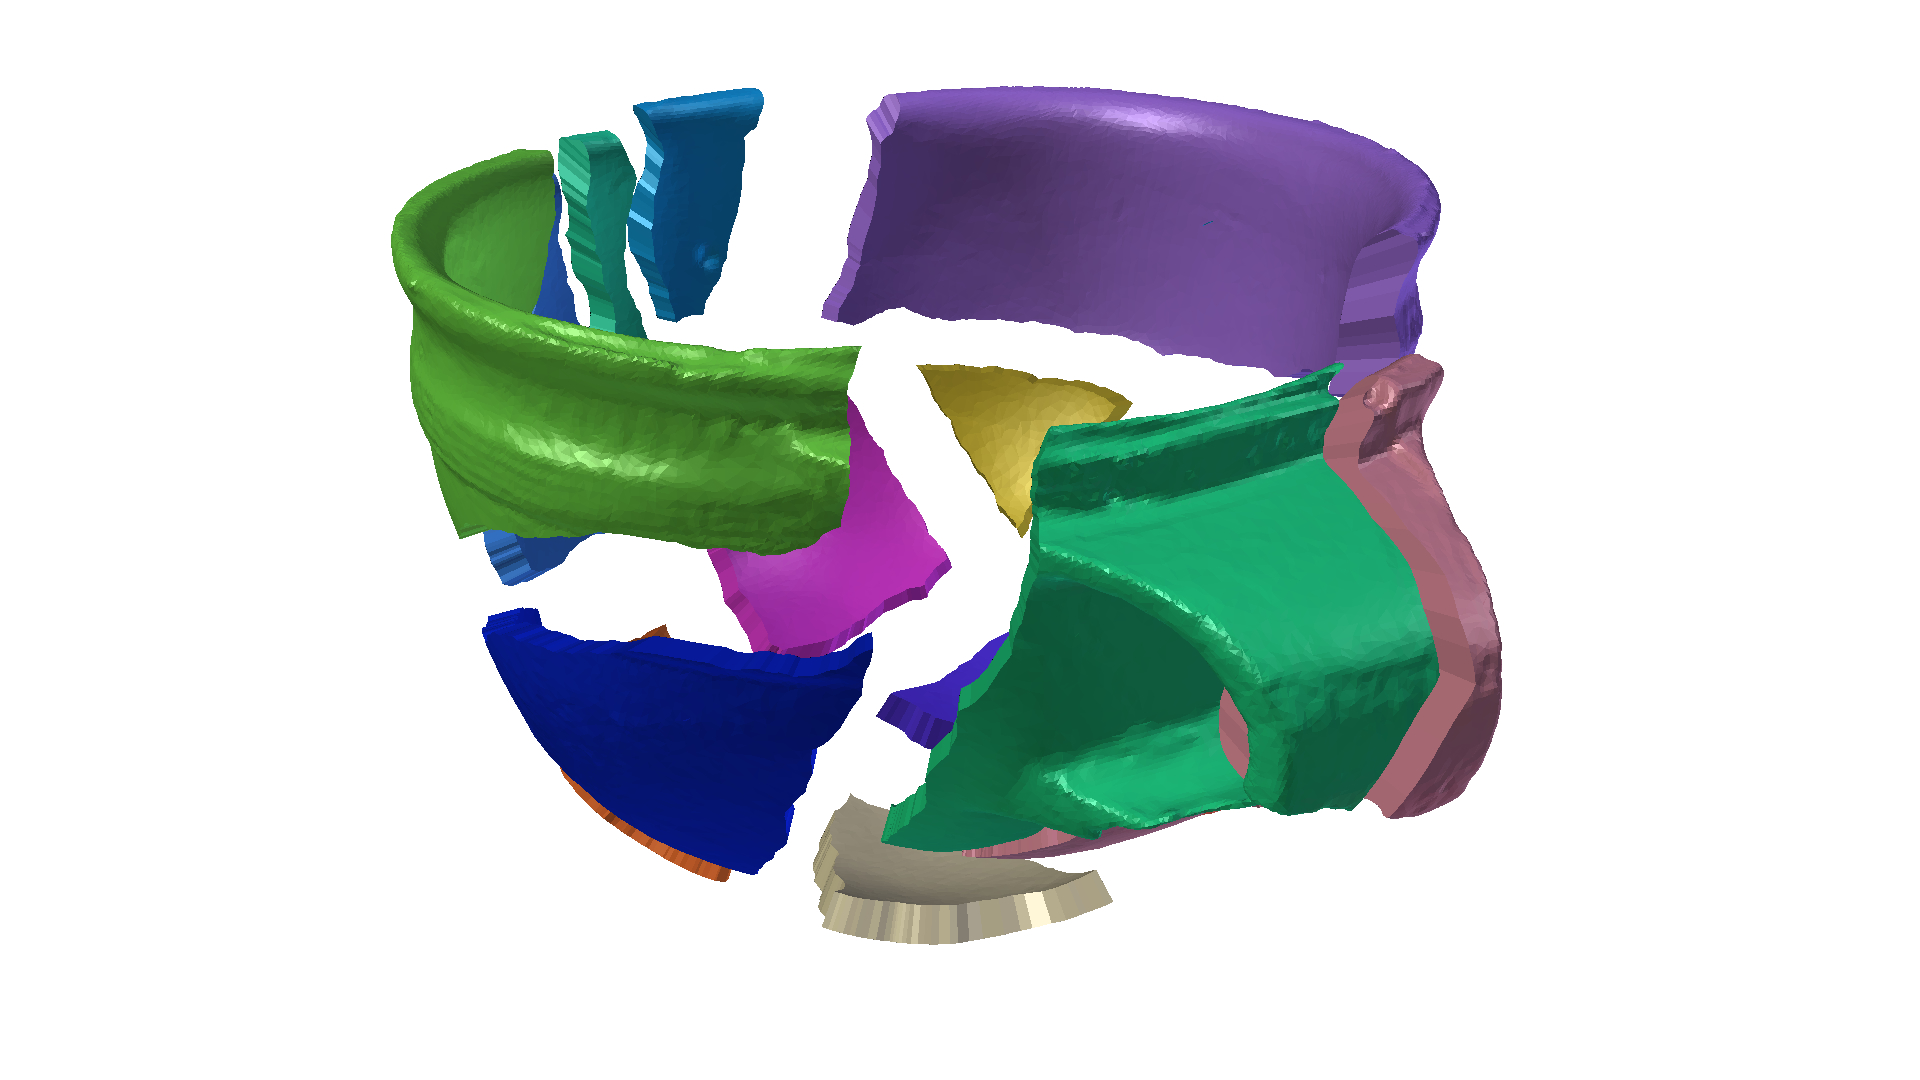
\includegraphics[width=0.33\textwidth]{images/ambercuppuzzle0}%
  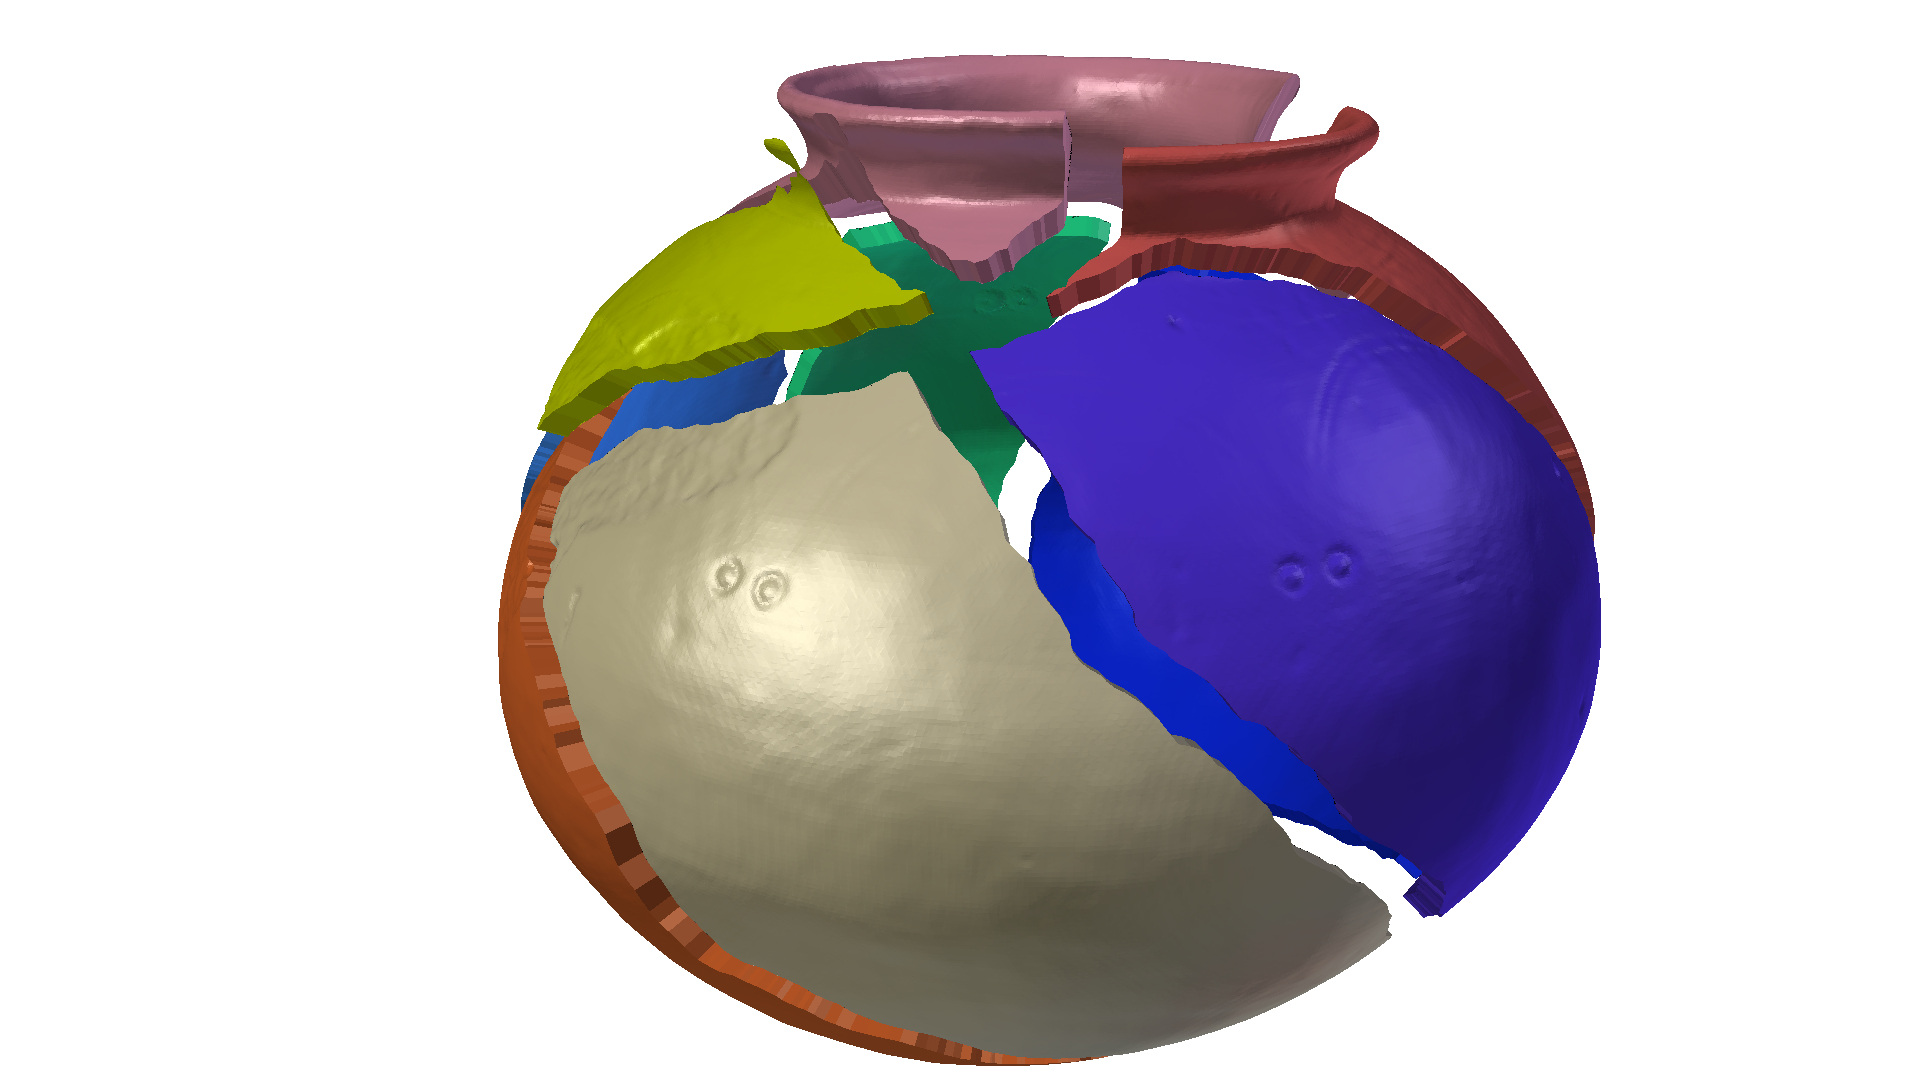
\includegraphics[width=0.33\textwidth]{images/saltdeanpuzzle0}%
  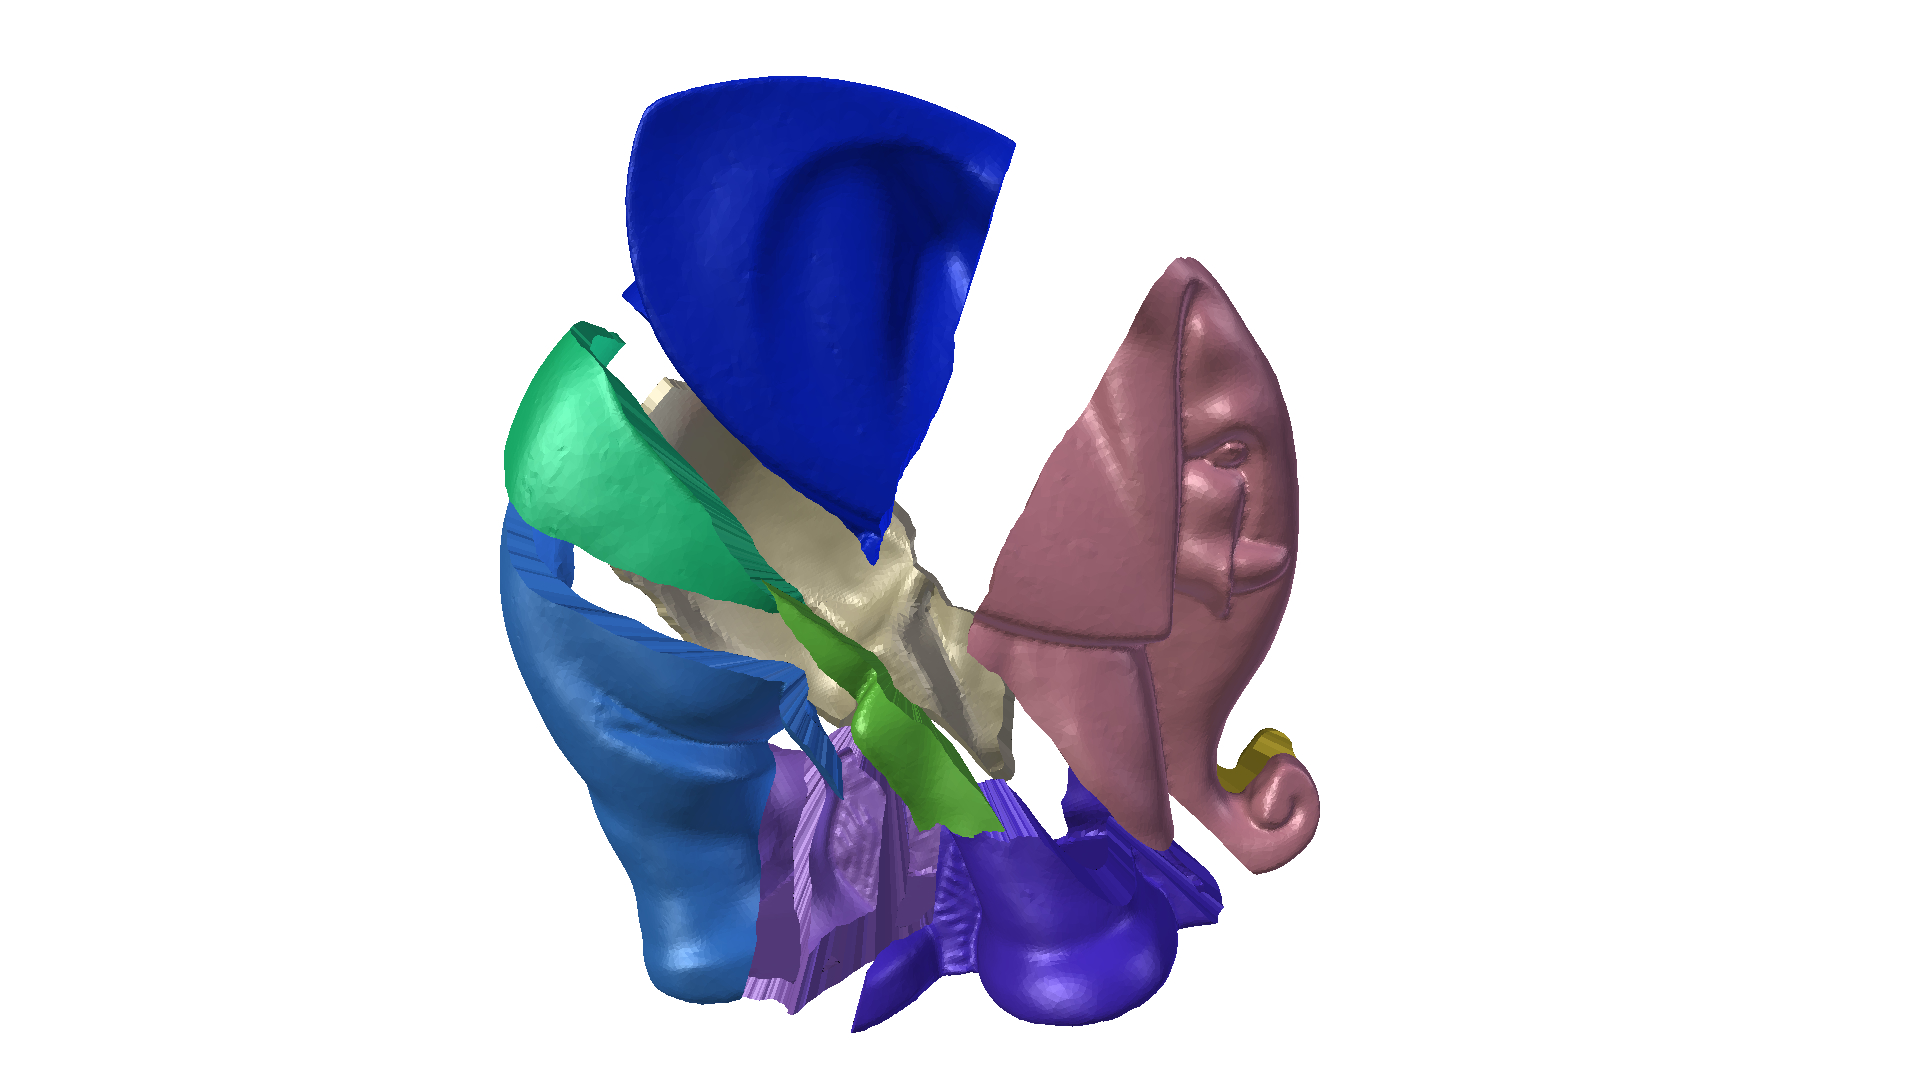
\includegraphics[width=0.33\textwidth]{images/elephantpuzzle0}\\
  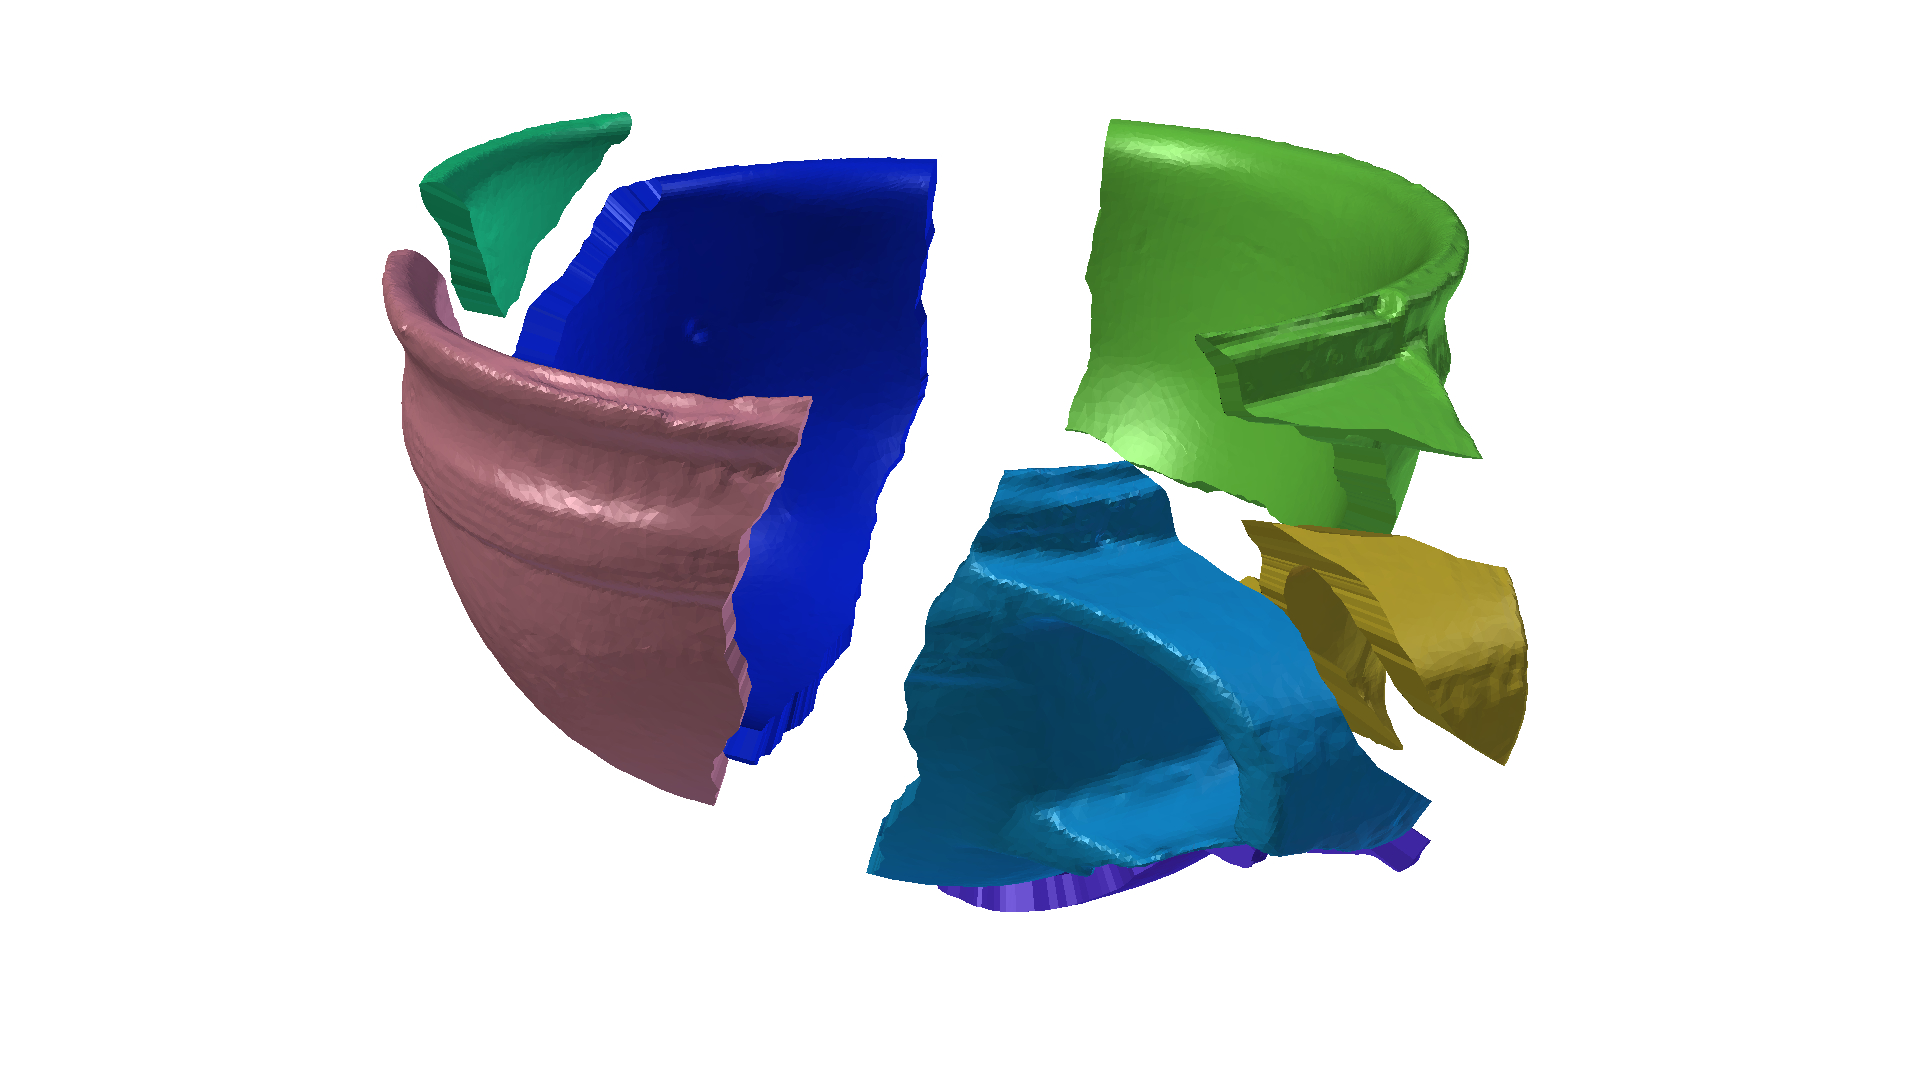
\includegraphics[width=0.33\textwidth]{images/ambercuppuzzle2}%
  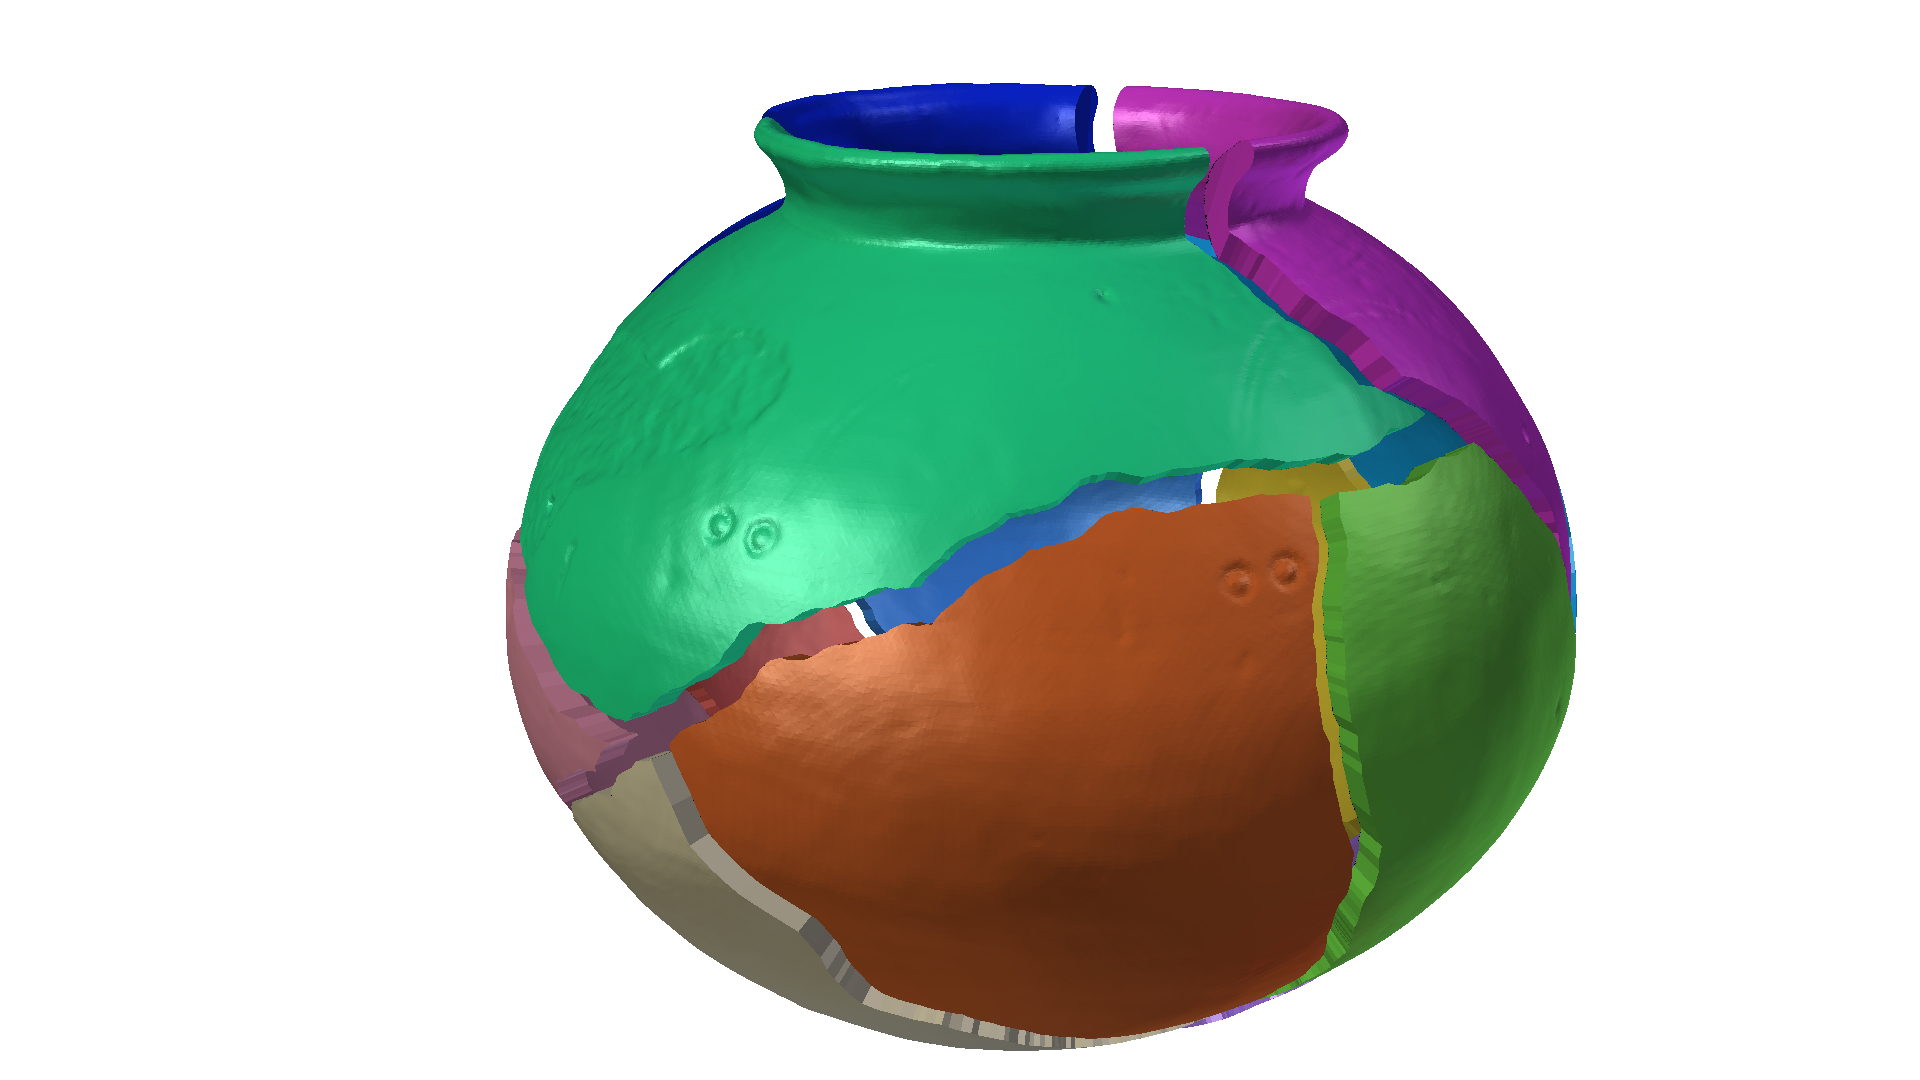
\includegraphics[width=0.33\textwidth]{images/saltdeanpuzzle1}%
  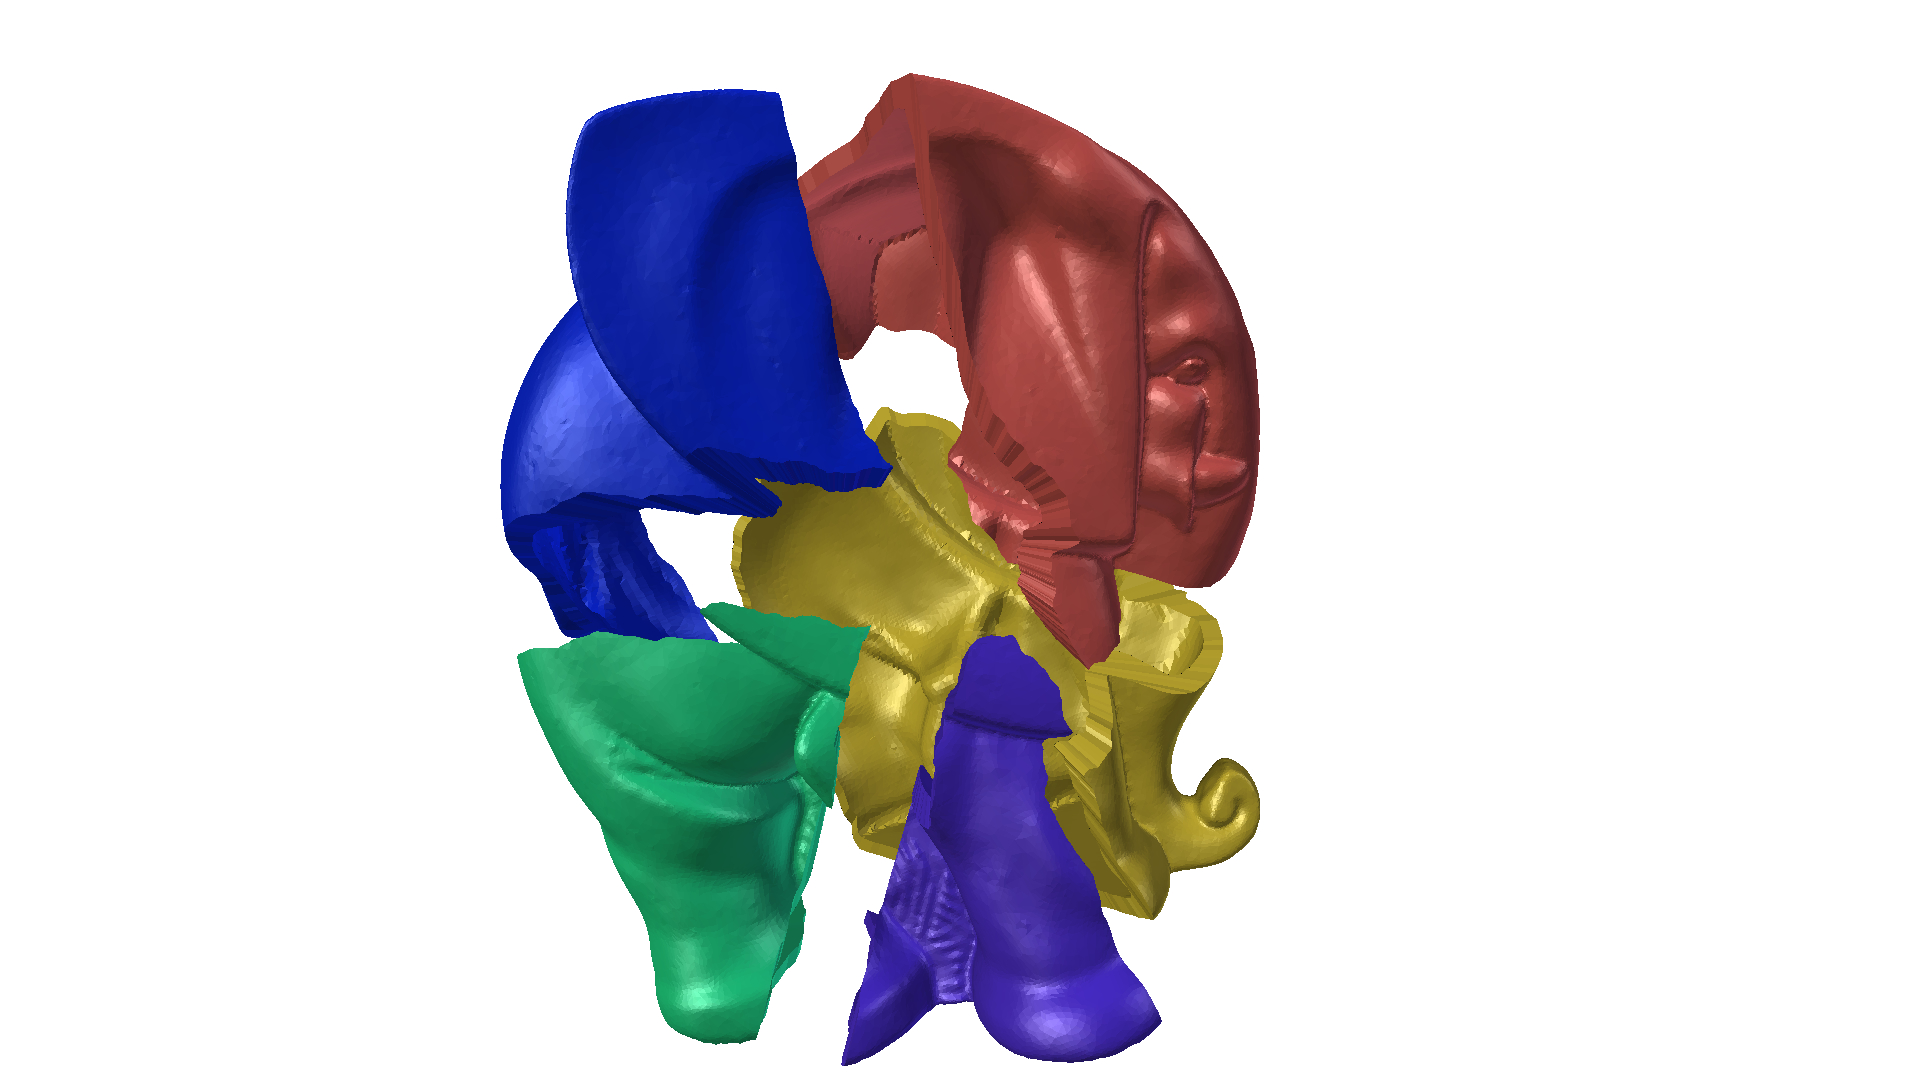
\includegraphics[width=0.33\textwidth]{images/elephantpuzzle1}\\
  %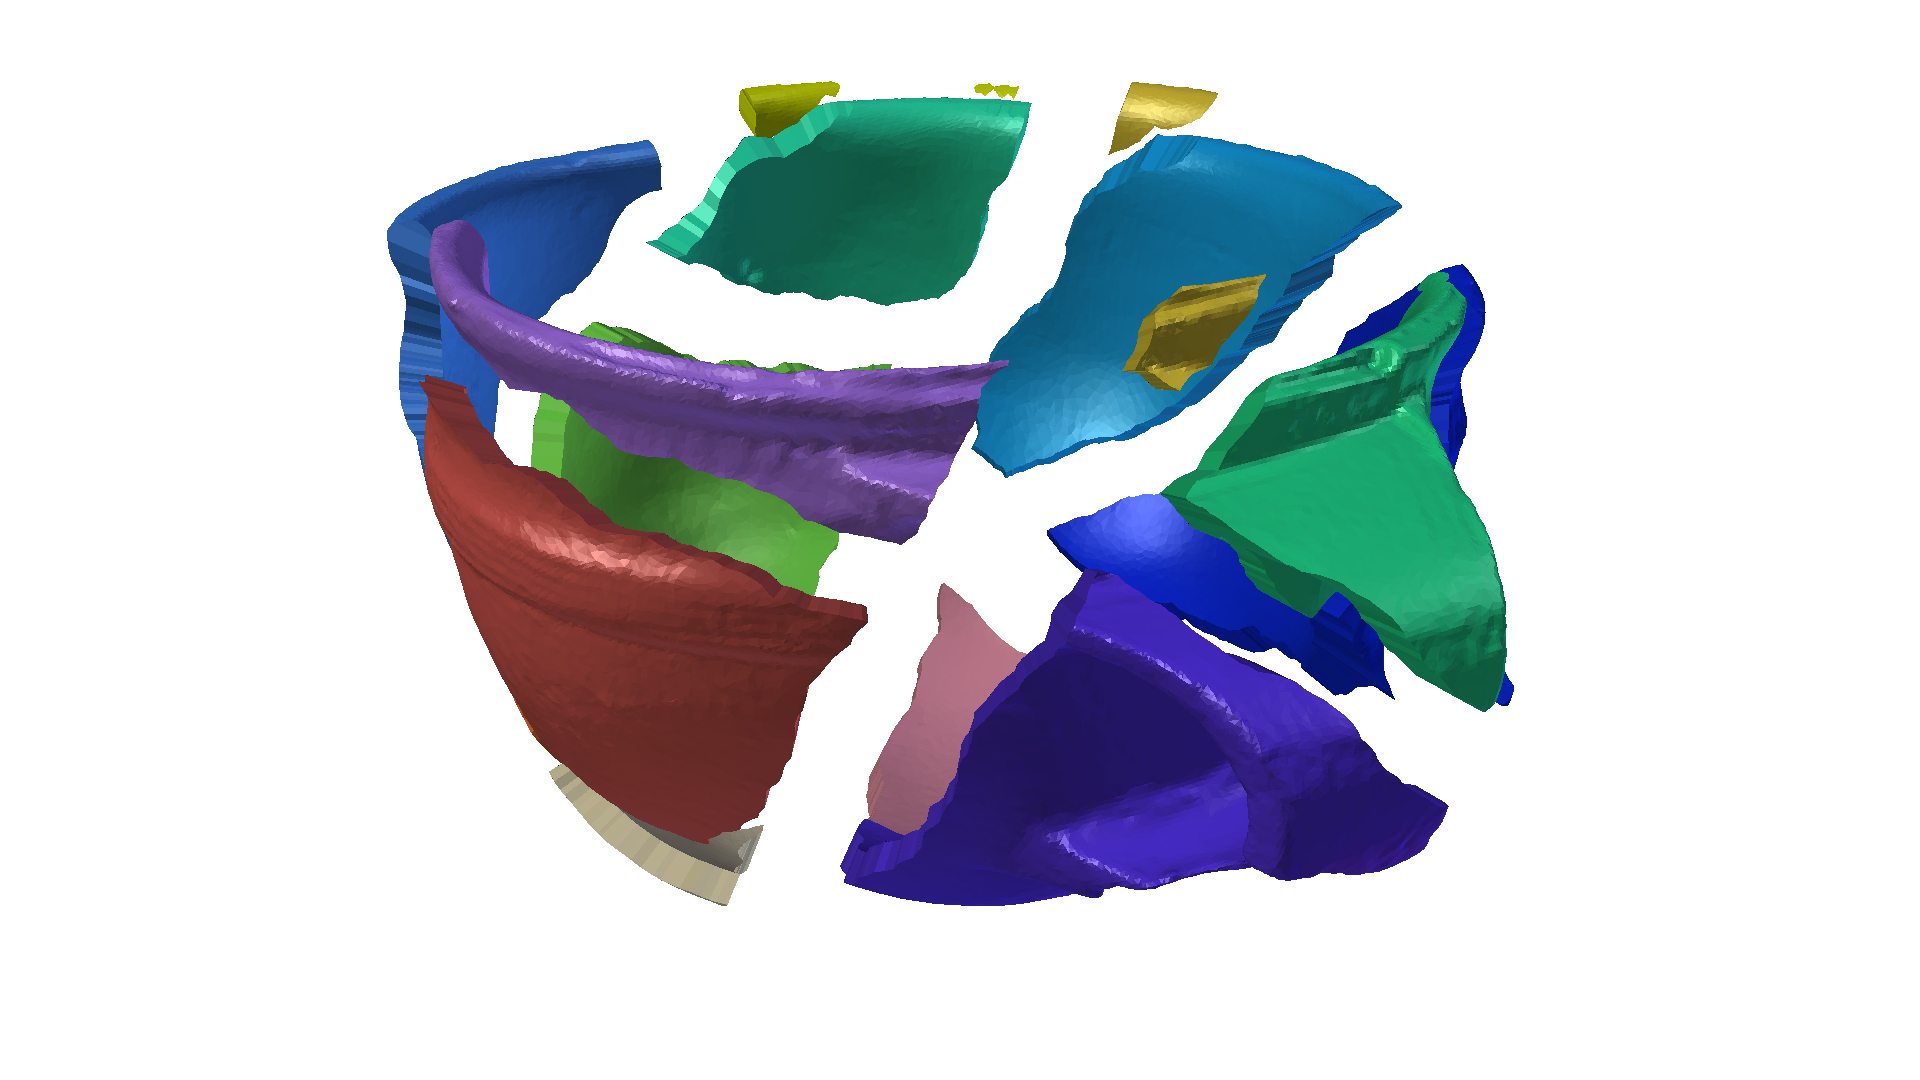
\includegraphics[width=0.55\textwidth]{ambercuppuzzle3}\\
  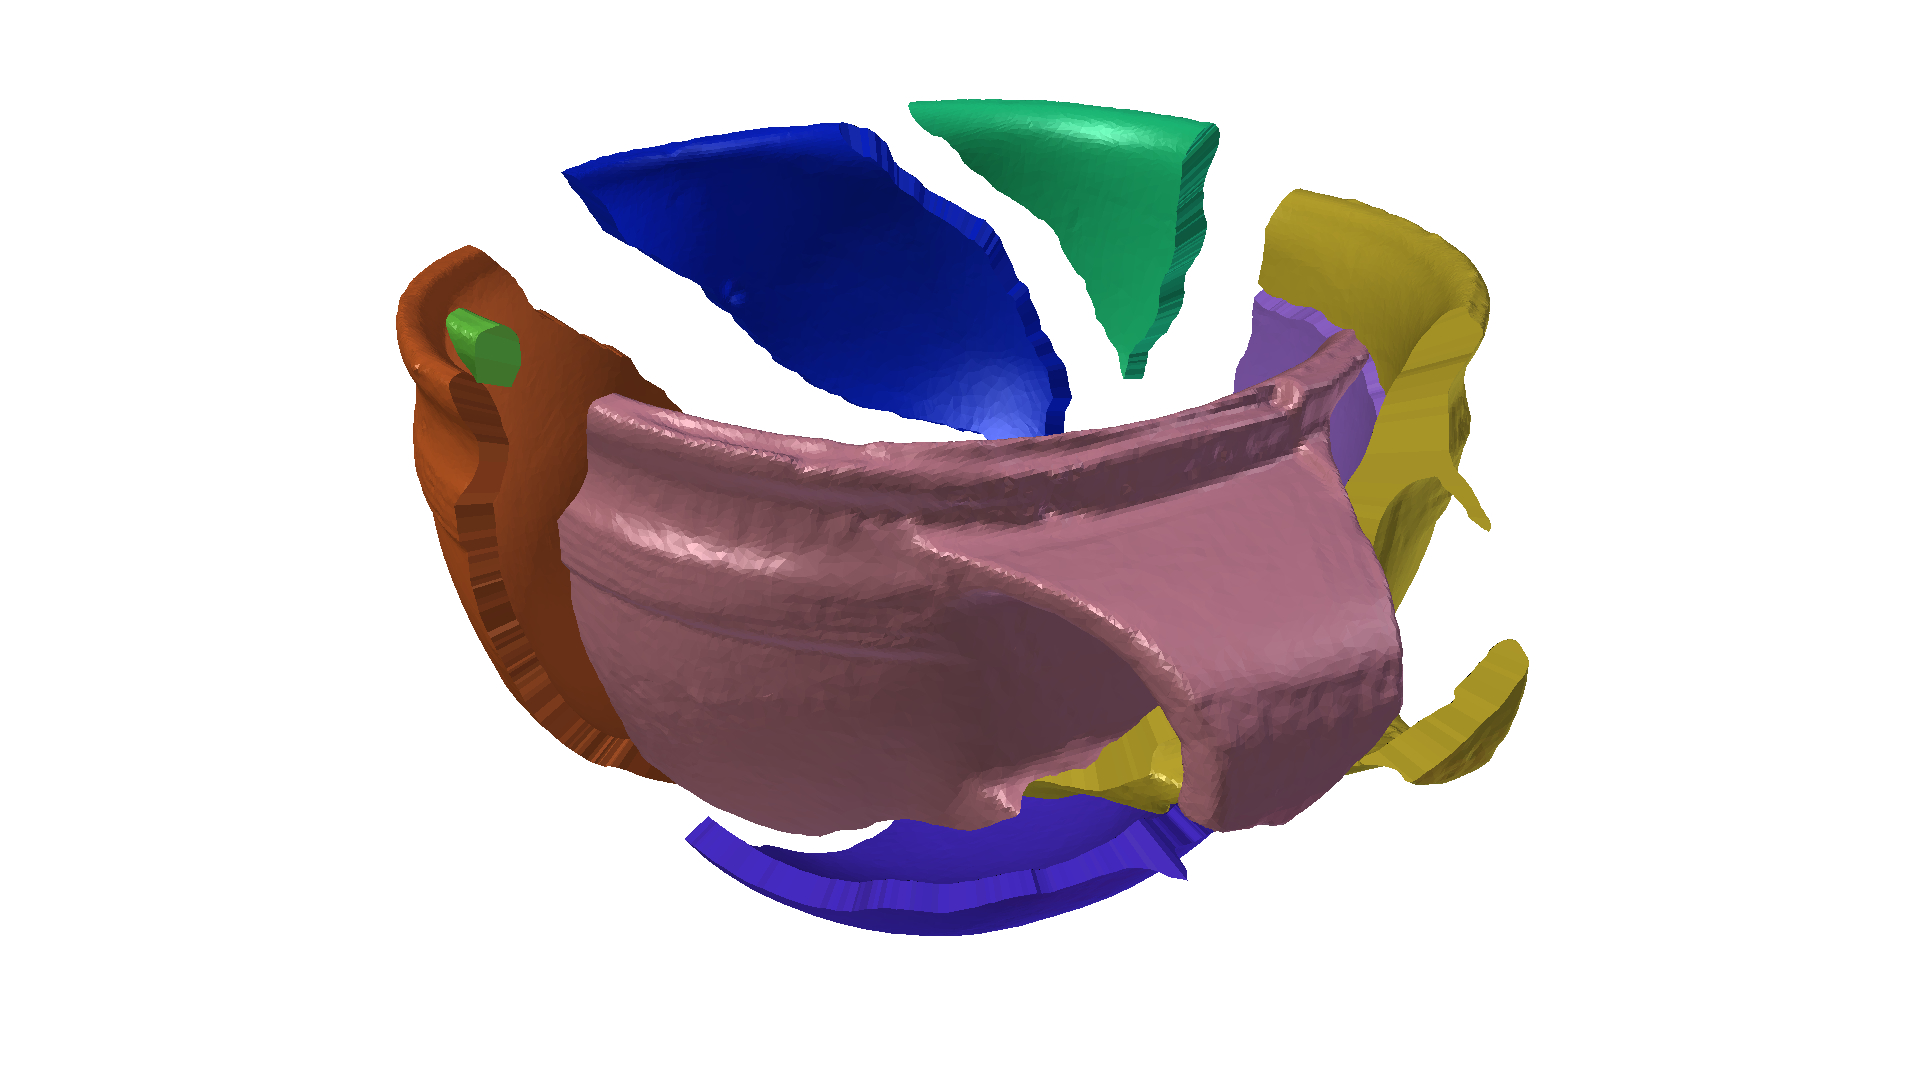
\includegraphics[width=0.33\textwidth]{images/ambercuppuzzle4}%
  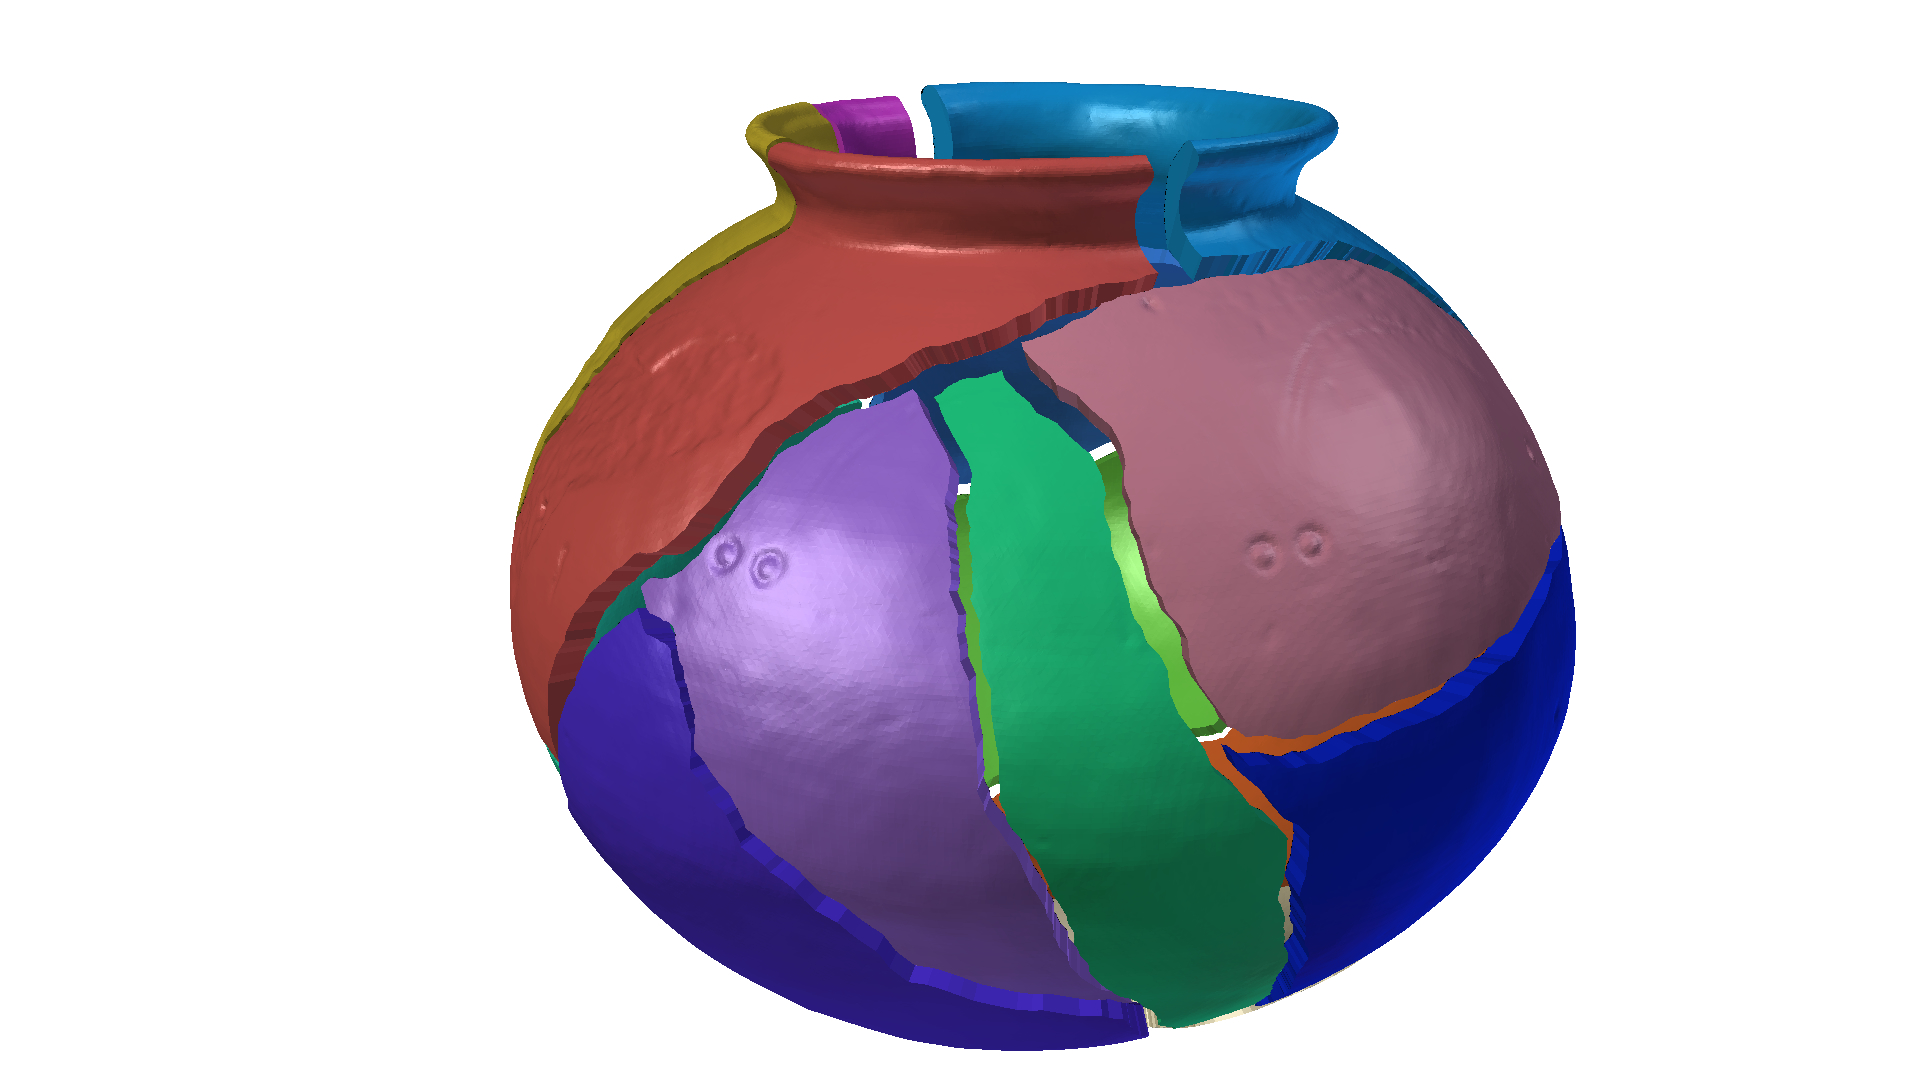
\includegraphics[width=0.33\textwidth]{images/saltdeanpuzzle2}%
  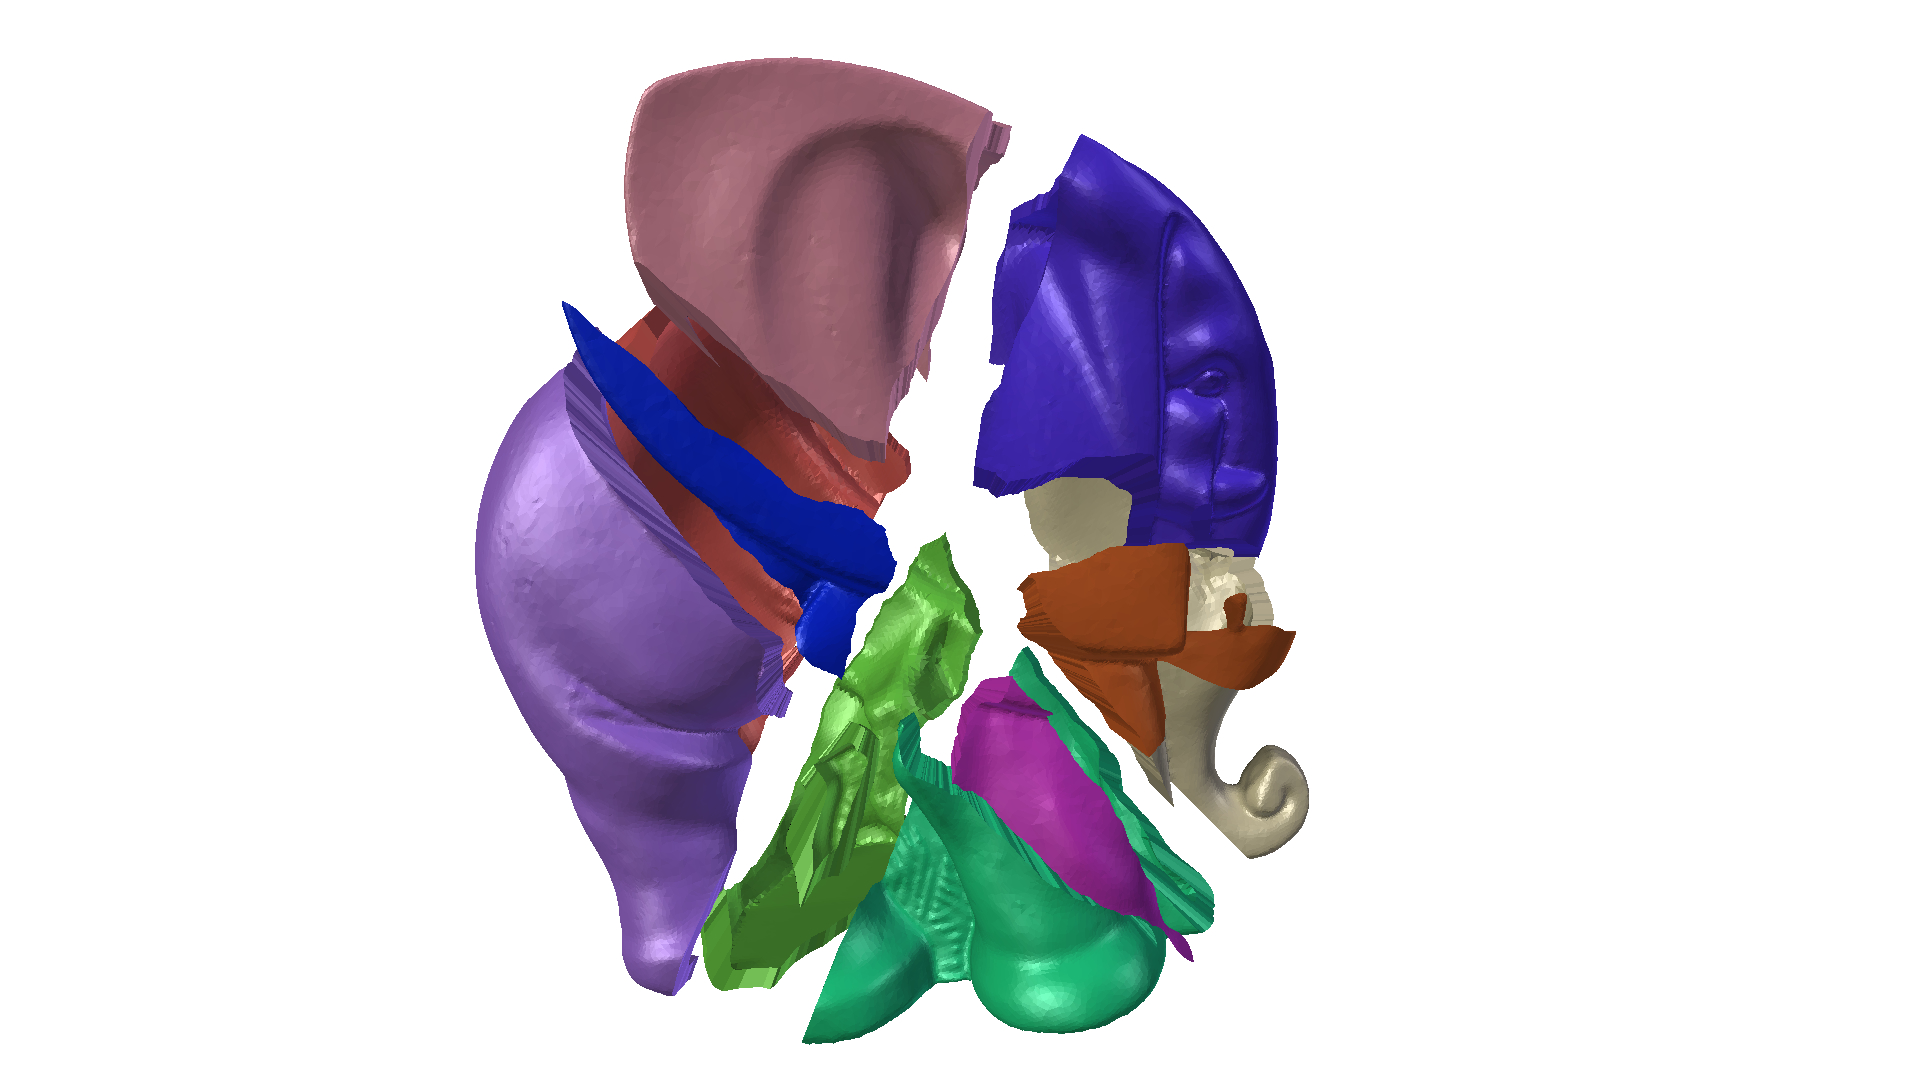
\includegraphics[width=0.33\textwidth]{images/elephantpuzzle2}\\
  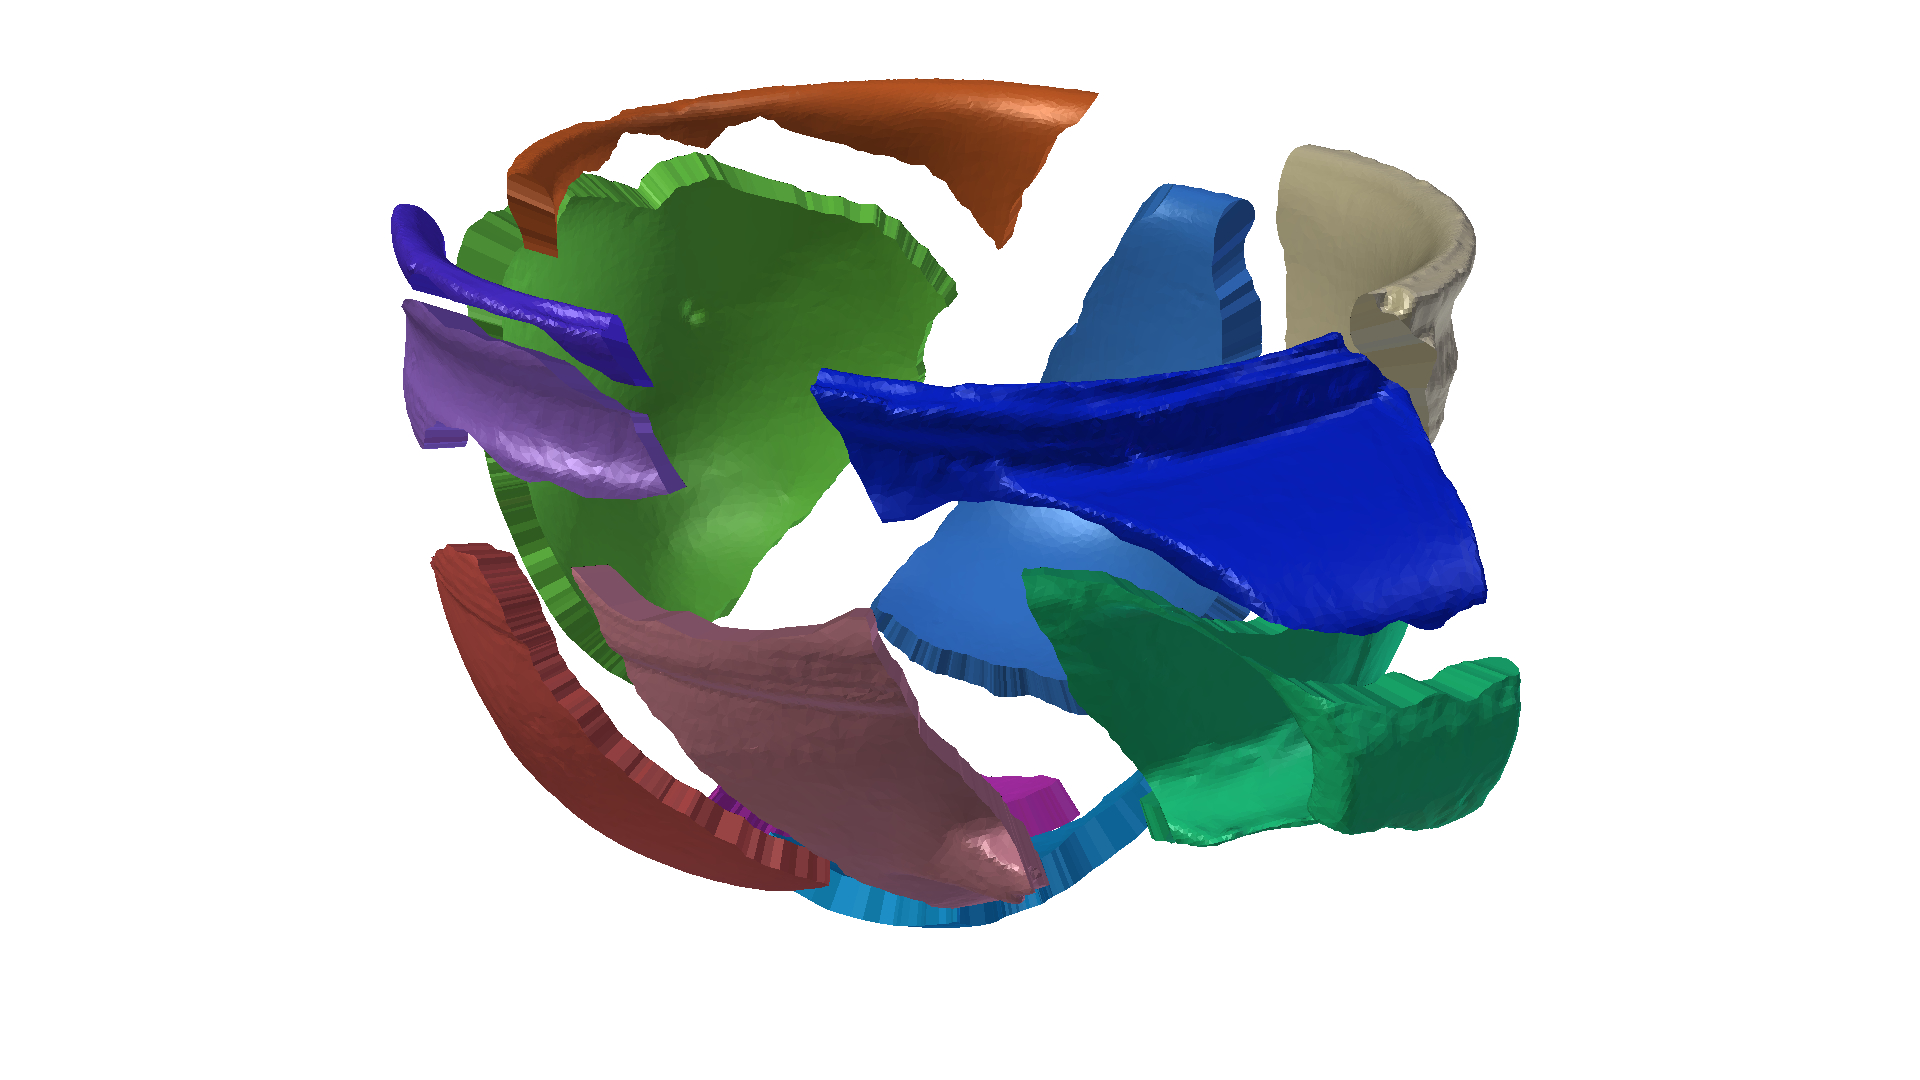
\includegraphics[width=0.33\textwidth]{images/ambercuppuzzle5}%
  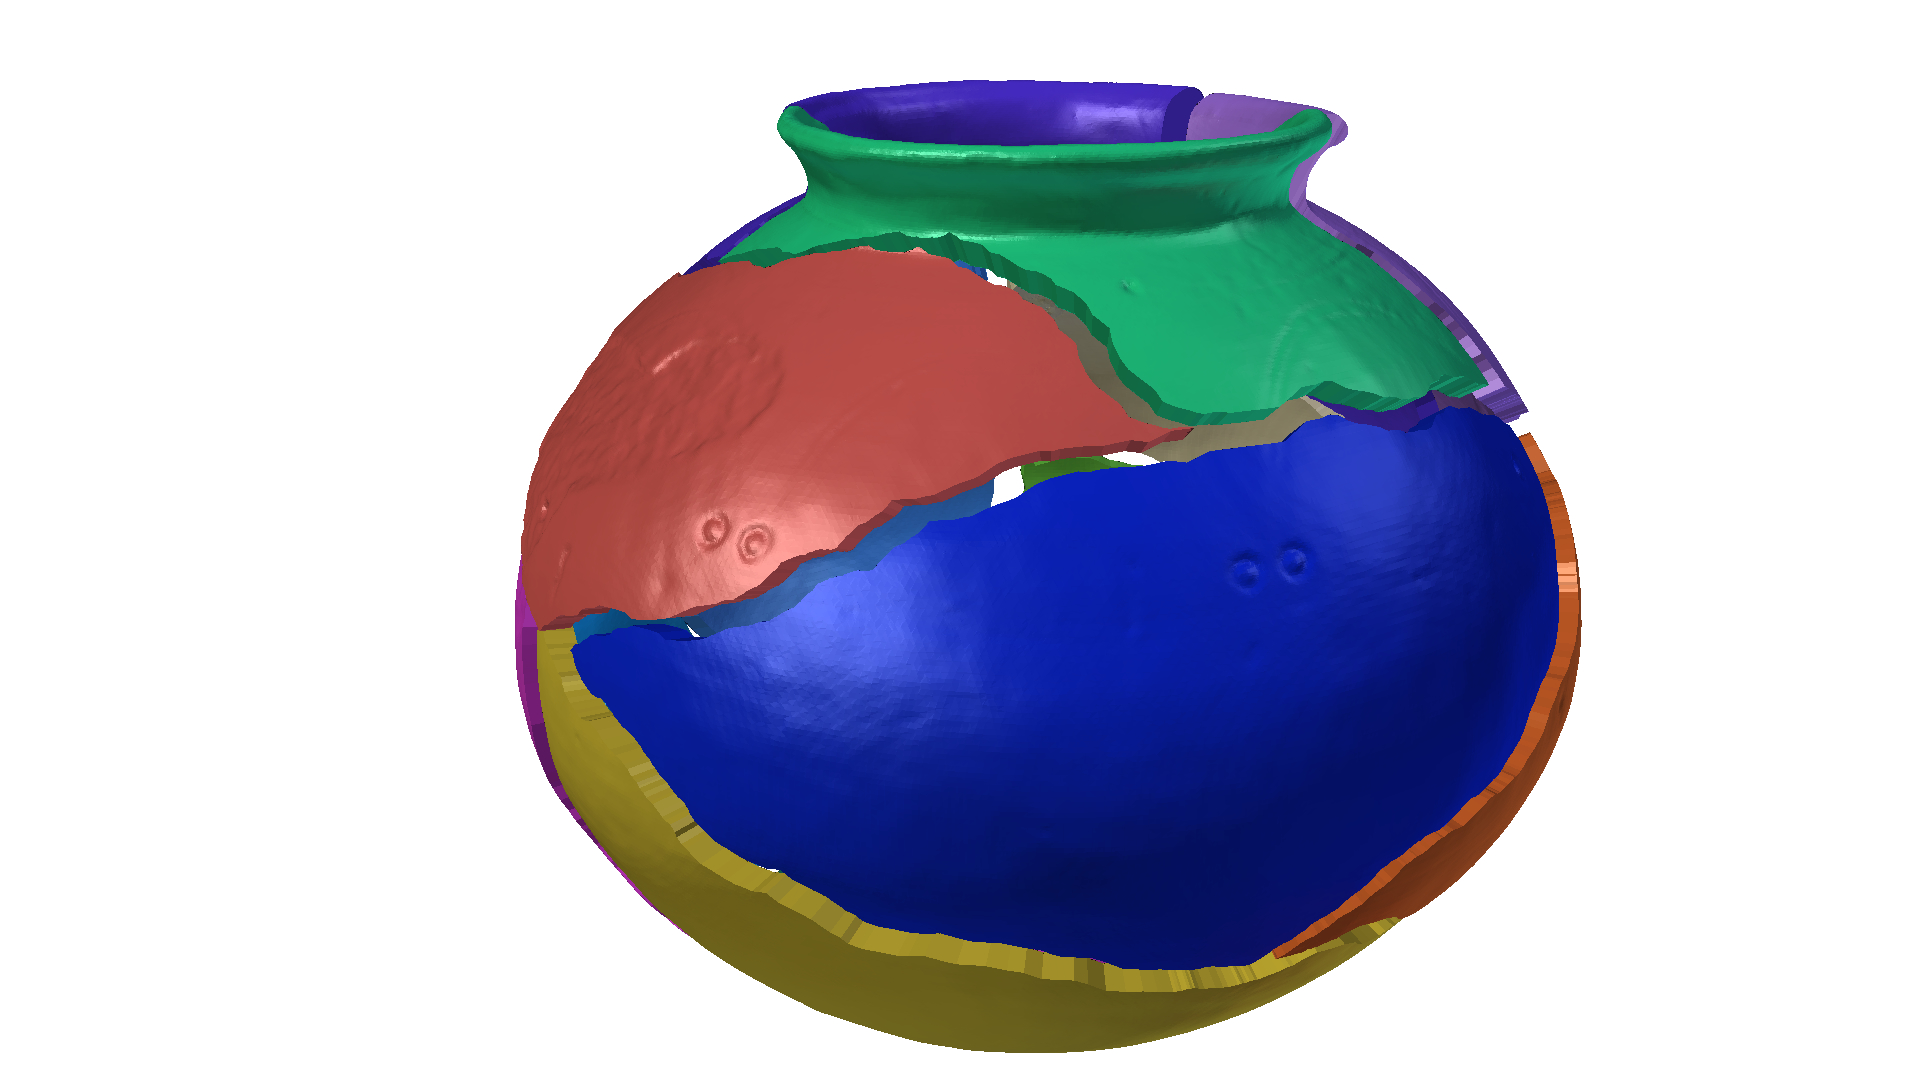
\includegraphics[width=0.33\textwidth]{images/saltdeanpuzzle3}%
  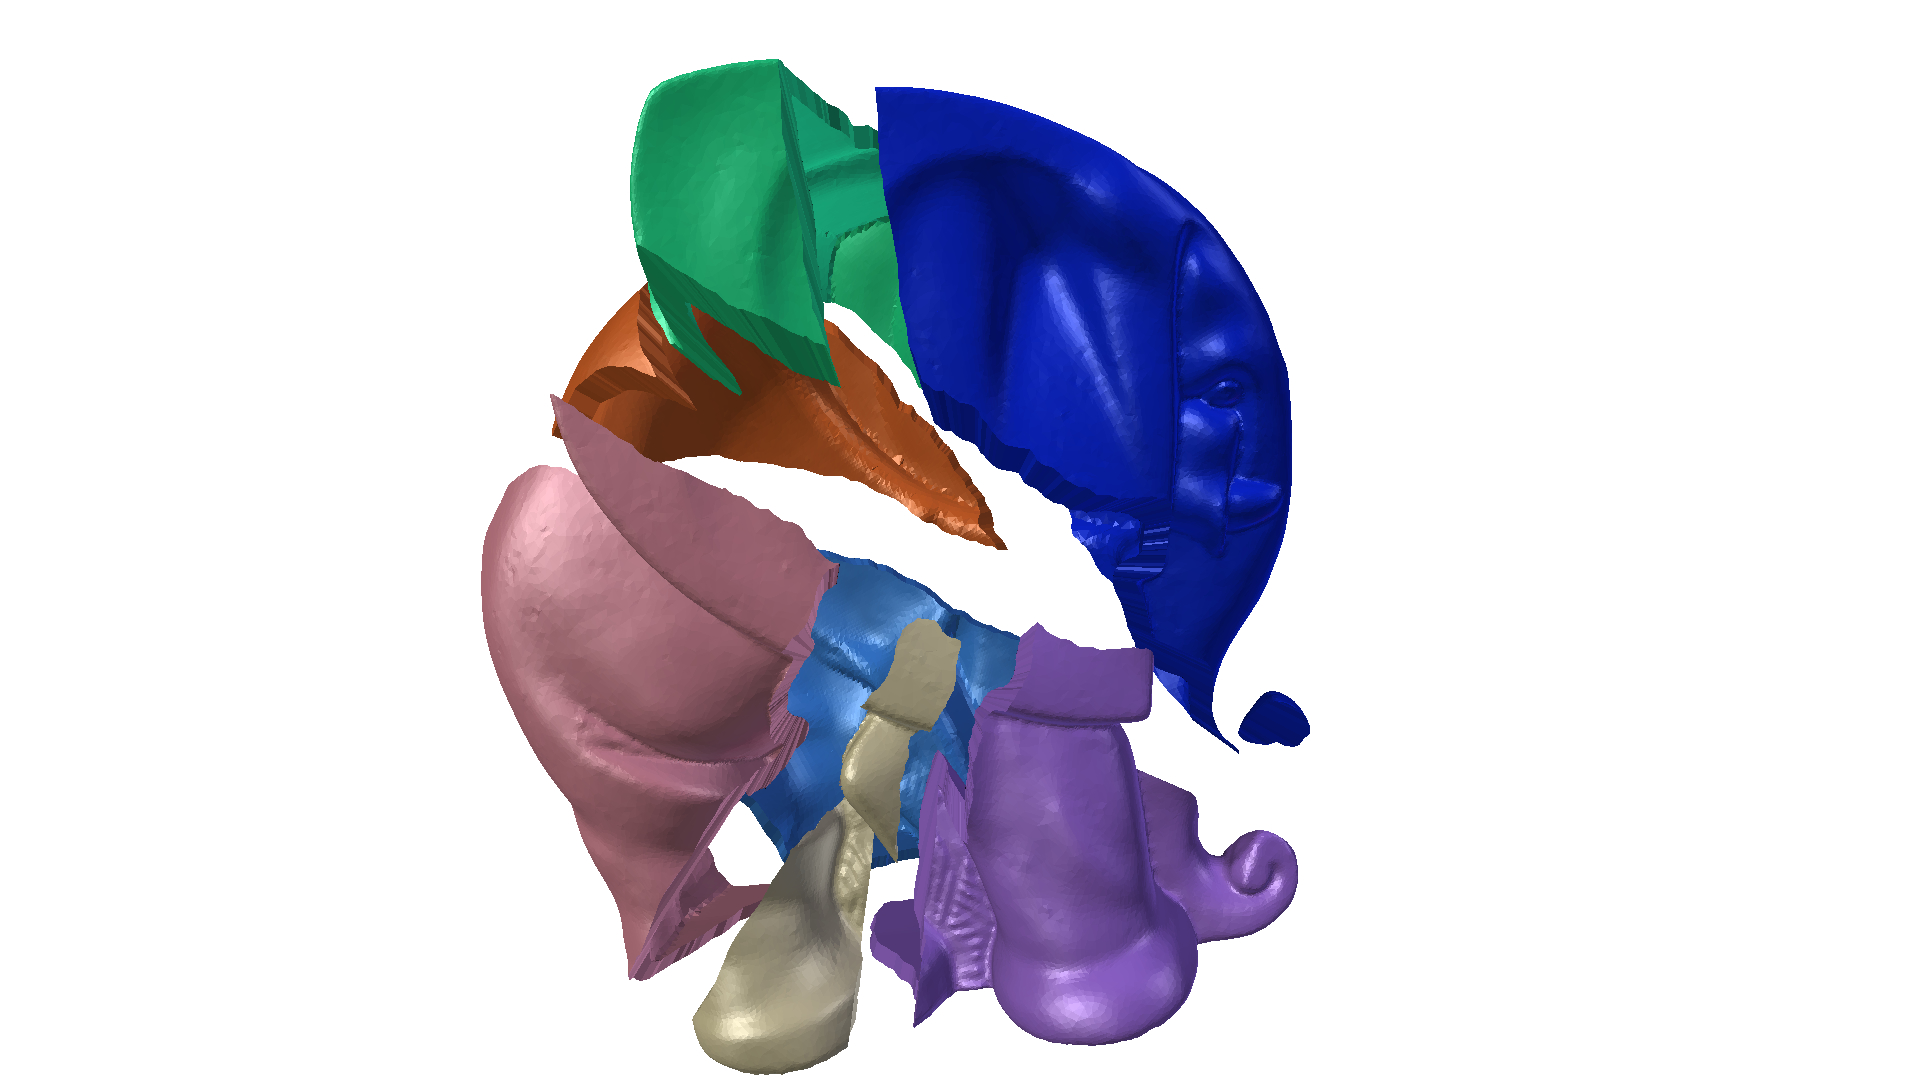
\includegraphics[width=0.33\textwidth]{images/elephantpuzzle3}\\
  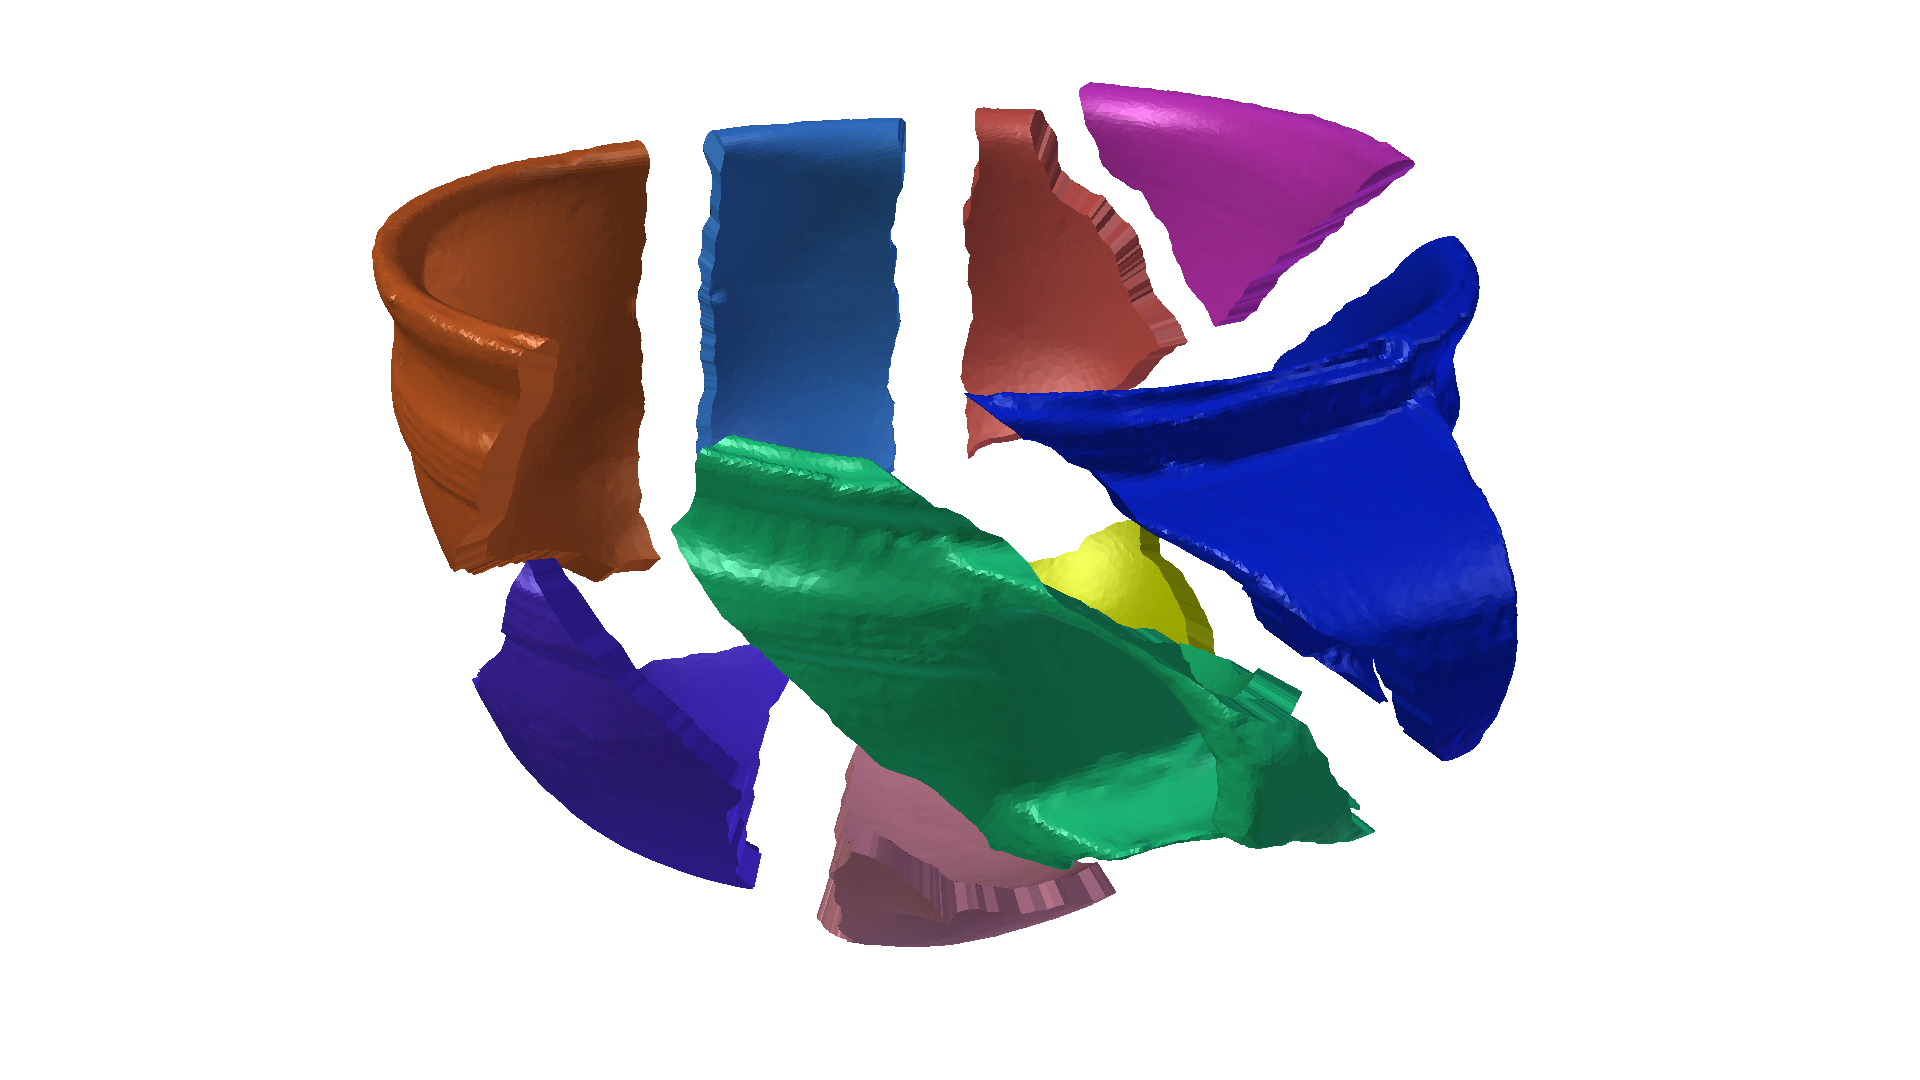
\includegraphics[width=0.33\textwidth]{images/ambercuppuzzle6}%
  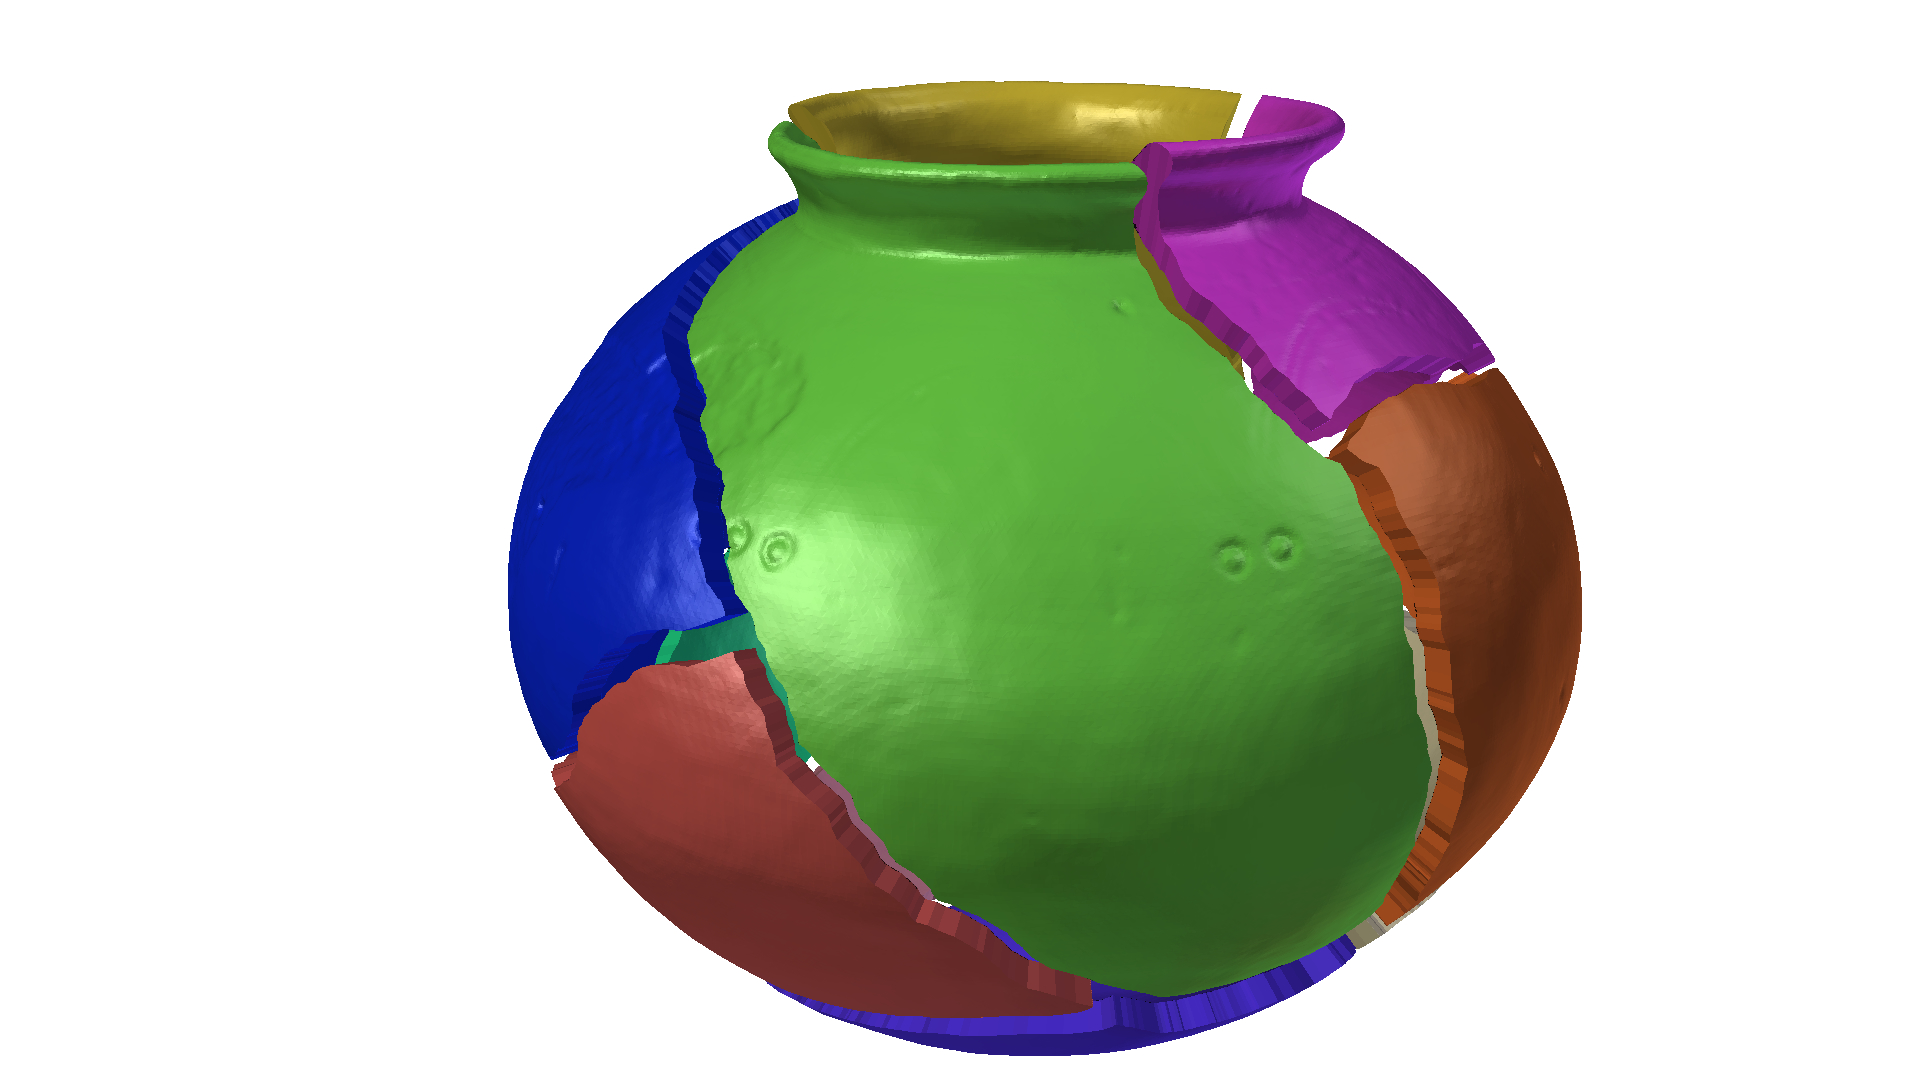
\includegraphics[width=0.33\textwidth]{images/saltdeanpuzzle4}%
  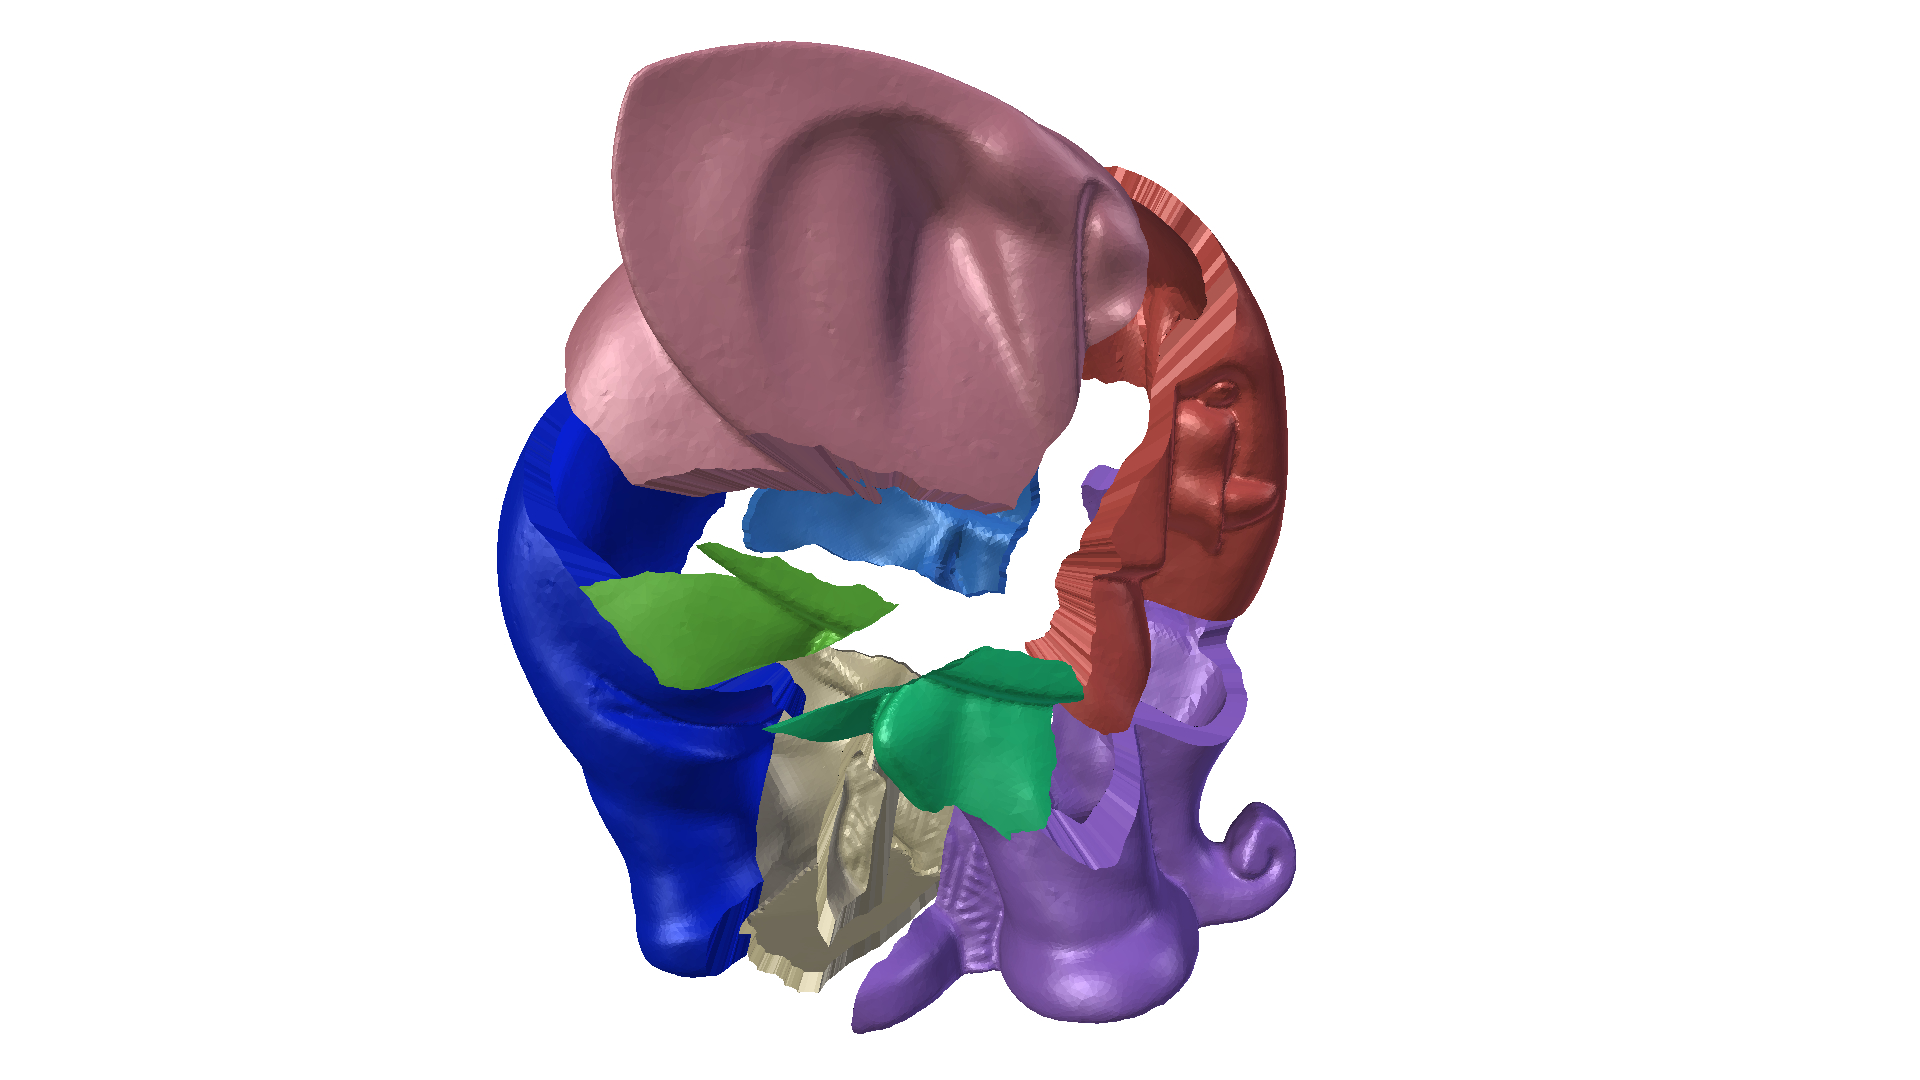
\includegraphics[width=0.33\textwidth]{images/elephantpuzzle4}
  \caption{Examples of algorithm applied to scans of an Amber cup, Saltdean pot and
    ceramic elephant figurine.}
\end{figure}

\begin{figure}[h]    
     \centering
      \subcaptionbox{m: 6, niter: 6, jitter: 0.3, amplitude: 0.1, decay: 0.5, smoothing: 0.0\label{normal}}
        {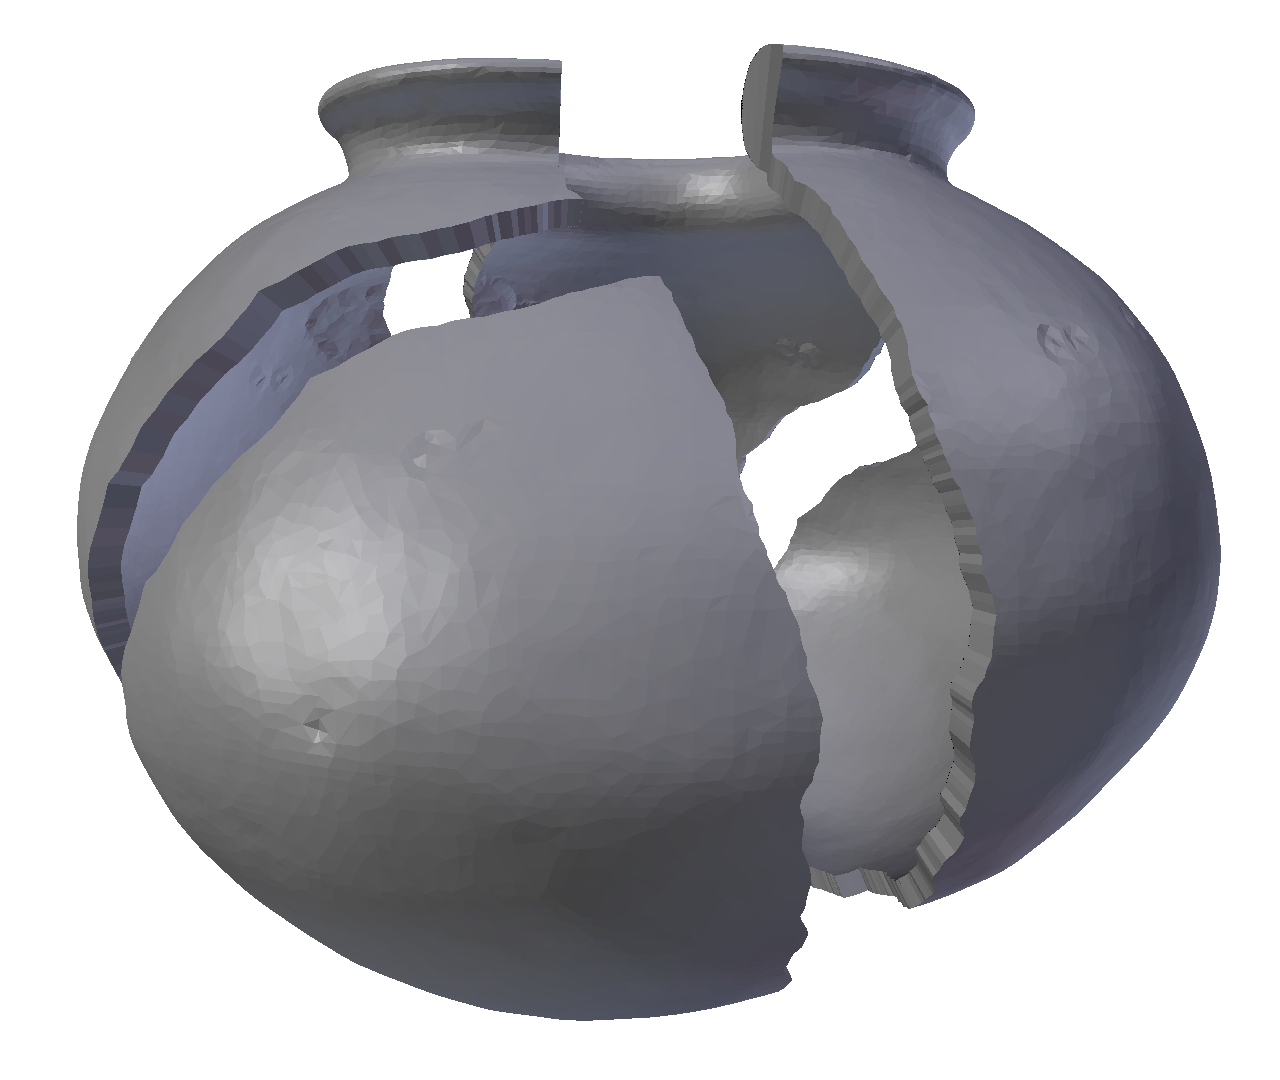
\includegraphics[width=0.33\textwidth]{images/all11.jpg}}
      \subcaptionbox{m: 6, niter: 6, jitter: 0.3, amplitude: 0.1, decay: 0.5, smoothing: 1.0\label{normalsmooth}}
        {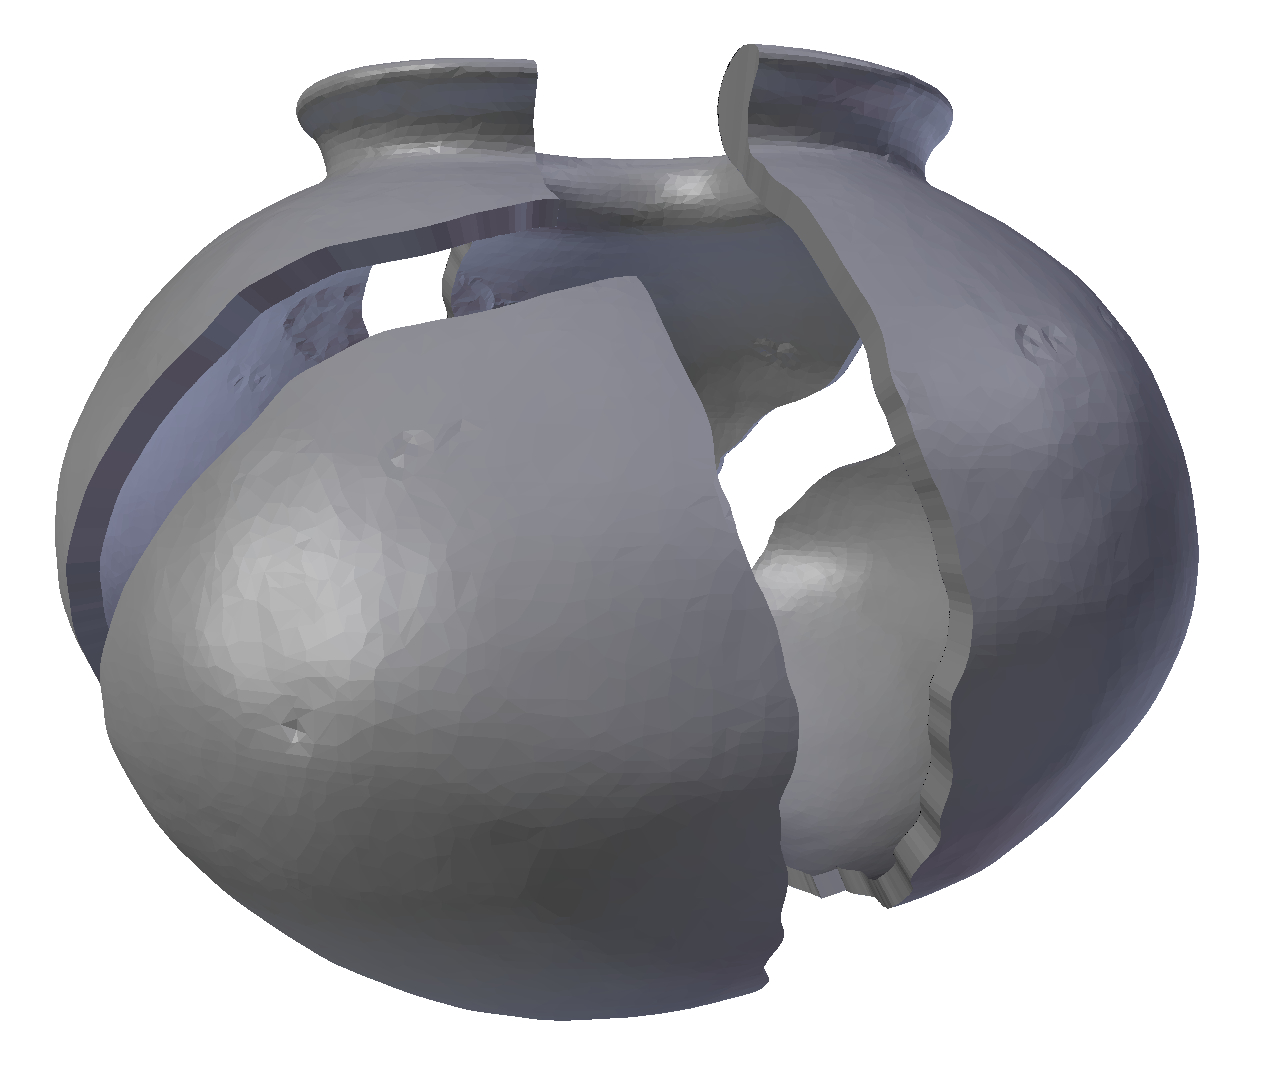
\includegraphics[width=0.33\textwidth]{images/all22.jpg}}
      \subcaptionbox{m: 6, niter: 6, jitter: 0.3, amplitude: 0.01, decay: 0.5, smoothing: 0.0\label{lowjitter}}
        {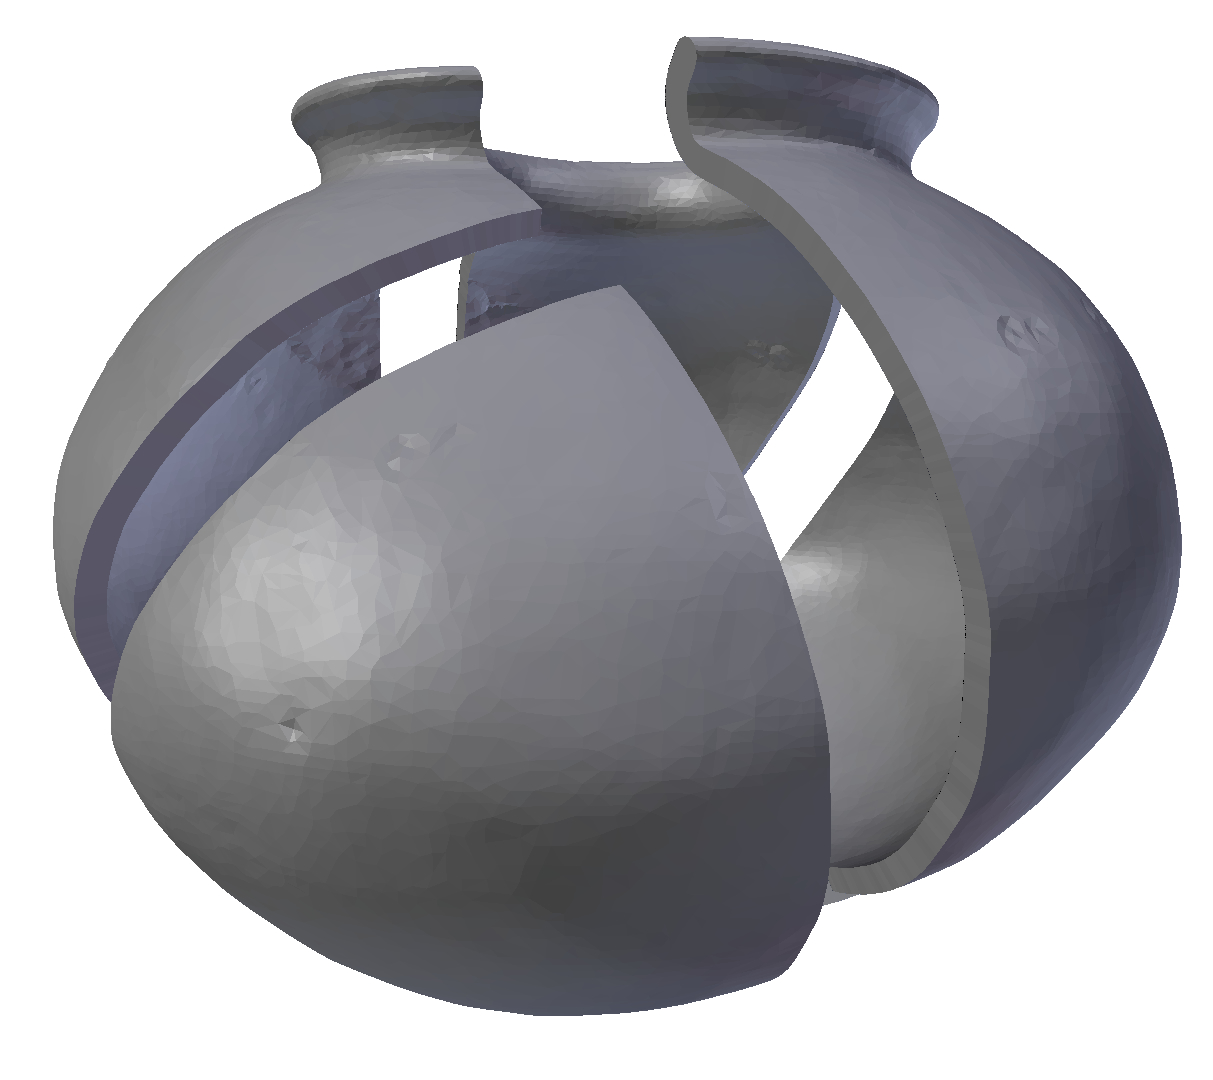
\includegraphics[width=0.33\textwidth]{images/all33.jpg}}
      \subcaptionbox{m: 6, niter: 6, jitter: 0.3, amplitude: 0.2, decay: 0.2, smoothing: 1.0t\label{highjitter}}
        {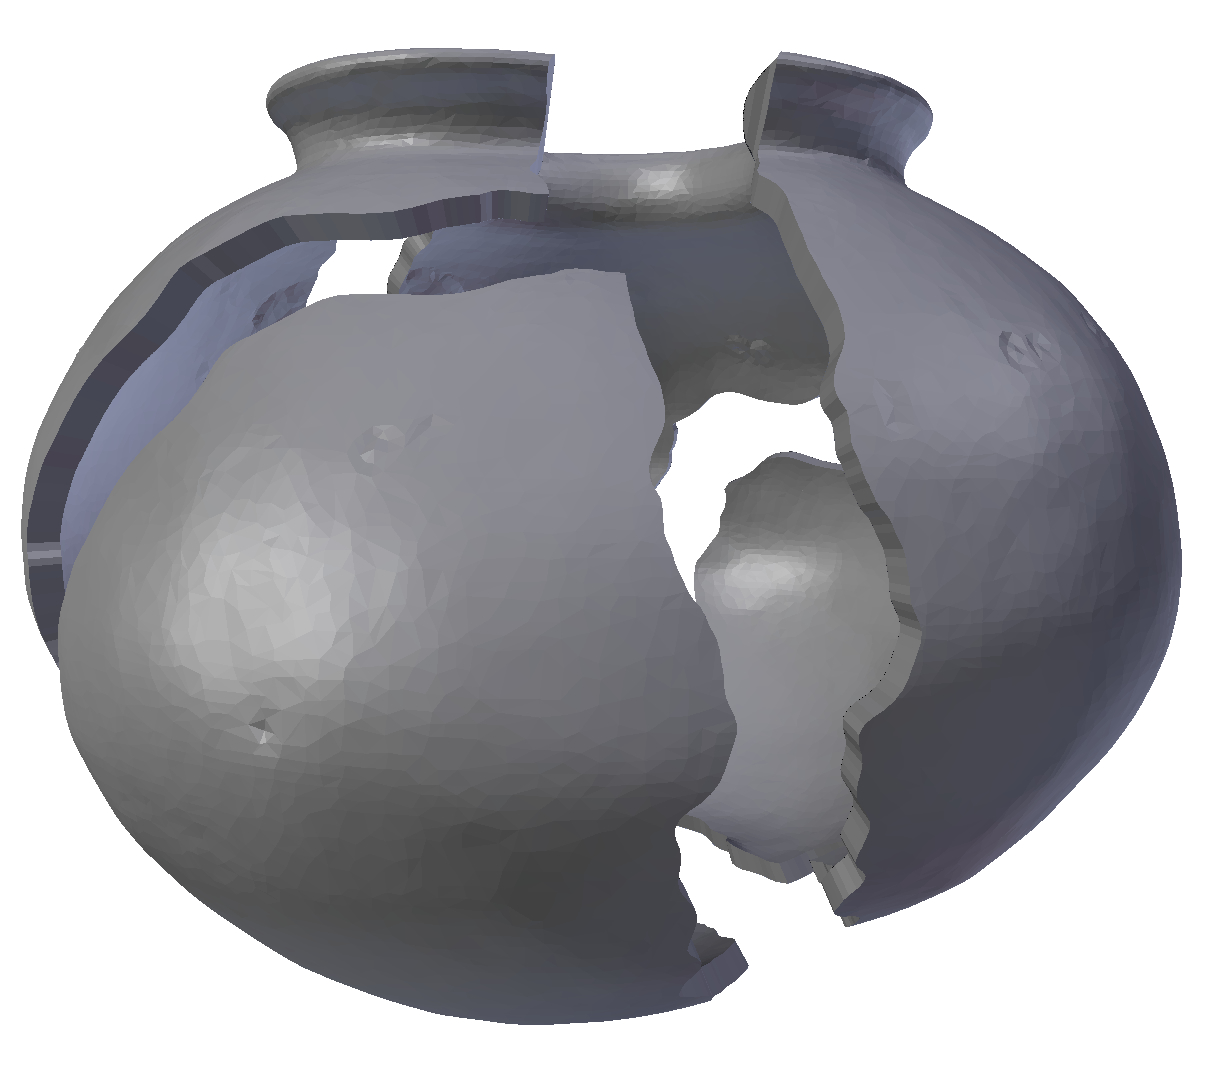
\includegraphics[width=0.33\textwidth]{images/all44.jpg}}
      \caption{Examples of puzzles with different parameters}\label{allsettings}
\end{figure}
\section{Evaluation}
\label{eva}

The puzzle, its design and performance have been mainly tested with
the design team and the curators of the museum. The functional testing
has been an iterative process throughout the digital fabrication
workflow to see whether the requirements of the activity/exhibit have
been met. The feedback from this process has informed design decisions
at subsequent steps of the workflow.

The evaluation of the puzzle pot activity and its performance in terms
of enhancing the visiting experience for families of the
Archaeological Gallery of the Brighton Museum and Art Gallery will
take place \KRedit[once the Gallery is open to the public]{as part of a larger research project on digitally fabricated interpretation material}. A detailed method
for the evaluation has already been set up and tested with another
museum~\cite{Samaroudi2017}.

A final consideration is given to how this solution compares to other
fabrication methods of archaeological puzzles. For instance, a similar
puzzle to the one produced could be made using a more traditional
approach: by modeling a pot from a hard wearing clay, firing and
glazing it. This pot could then be smashed, reassembled and a core
could then be made. This process is not very expensive, as it would
probably cost one third of the cost of our proposed approach, and also
requires only access to clay and a kiln. However, the puzzle pieces
would not have very good quality. For instance, the pieces would not
necessarily break with the dimensions required and in equal sizes, the
magnets would be difficult to fit neatly. Most importantly, if a
single piece disappeared from the gallery, the process to replace the
piece would be costly and complex.

Alternatively, it is possible to make a pot using clay and produce a
mould or negative using plaster of Paris or silicone. Tin would then
be used to make the shard shapes in the mould. The puzzle pieces and
core would then be casted in jesmonite. Holes for the magnets would
then be drilled in the casted material. Although this process is
slightly more expensive than the previous one, it would be possible to
replace a piece if this was lost. However, the mould would require to
be carefully guarded so it does not get lost, and it would suffer of
inevitable wear out. The latter issue would affect the reproduction of
subsequent copies of puzzle pieces.

The proposed approach has the following advantages in relation to the
previous approaches: i) it uses an authentic artefact of the
collection, ii) it is far simpler and more cost-effective making
multiple copies or replacements once the digital design and testing is
done, iii) it allows the generation of puzzles of other shapes and
sizes in a more cost-effective way, and iv) the digital model is a
valuable outcome by itself, for instance it can be used in interactive
puzzle-making applications on the web and can be shared with other
museums in case they wanted to replicate the physical experience.

%A small-scale pre-user acceptance test has also taken place with two
%children belonging to the age target group of the activity (6-12
%years old) to identify whether they can assemble parts of the
%puzzle. Initial testing has shown that the activity seems interesting
%for children who dedicate time happily to assemble the puzzle pot.

\section{Discussion and conclusions}
\label{conclusions}

This paper presented a novel digital workflow for the generation of 3D
puzzles for museum galleries. The workflow was deployed with a
particular artefact, the Saltdean urn. The 3D puzzle activity \KRedit[will be
exhibited]{is part of the archaeology gallery} at the Brighton Museum and Art Gallery.

The proposed workflow's input is an artefact which is digitised and
converted into a digital format. A series of steps are then employed
in order to produce a watertight model of the artefact and a core for
the puzzle pieces to ``sit on''. \KRedit{We then explore alternative fracture patterns in order to generate different types of puzzle pieces}. An algorithm is then proposed to
generate the puzzle fragments or shards and the \KRedit{attachments, such as} blind-holes for the
magnets on the pieces and core. \KRedit[These steps make use of a combination
of cell fracture algorithms and the Boolean operations provided by CAD
systems.]

\KR{we need to rephrase this, as I don't think these really are the greatest challenges.... the challenge really is the fabrication.}One of the challenges of the workflow is producing the watertight 3D
mesh suitable for the generation of the puzzle. This is because this
3D mesh is not a straight-forward outcome from the digitisation
processes. Due to these challenges, the urn's shape had to be
reconstructed to a certain extent to fill-in gaps which the
digitisation process did not capture, such as parts of the rim and the
inner-surface. The shape was also slightly simplified to make it
easier to handle in the modeling stage. The fabrication process also
requires considering tolerances due to the layer size of the 3D
printing technology.

The significance of the proposed workflow is that it can provide a CH
organisation with a cost-effective ``future-proof'' solution. Hence,
the process can be easily repeated either to replace lost pieces of
the puzzle or replicate the whole exhibit with minor
changes. Moreover, the presented process is relatively low cost in
comparison to other traditional design and production methods and can
be deployed to enhance the interpretation of artefacts in heritage
environments.

Future work will examine the effect that such an object and activity
have in engaging young audiences as well as investigating the
audience's opinion about the physical characteristics of the puzzle.

\section{Acknowledgments}

We thank the Brighton Museum and Art Gallery, and in particular Alex
Hawkey and Andrew Maxted, for their input and support during the
development of the research.

%
% The next two lines define the bibliography style to be used, and the bibliography file.
\bibliographystyle{ACM-Reference-Format}
\bibliography{sample-base}

\end{document}
